\chapter{Large scale solar power plants}
Almost all power that we use on our planet comes from the sun. Direct in form of radiation or indirect during wind, water and vegetation. Also the fossil power resources and reserves are stored energy from the sun in from of organic carbon compounds. There are two main technologies for generating electricity out of direct sun radiation. One is the direct conversion of solar irradiance to electrical energy while using photovoltaic. The other is to generate heat and convert it to electrical power. Figure~\ref{OverviewSTP} gives an abstract of the common technologies using direct solar power to generating electric power. This chapter has the focus on large-scale solar power plants and describes parts from both technologies.
\begin{figure}[!h] 
\centering
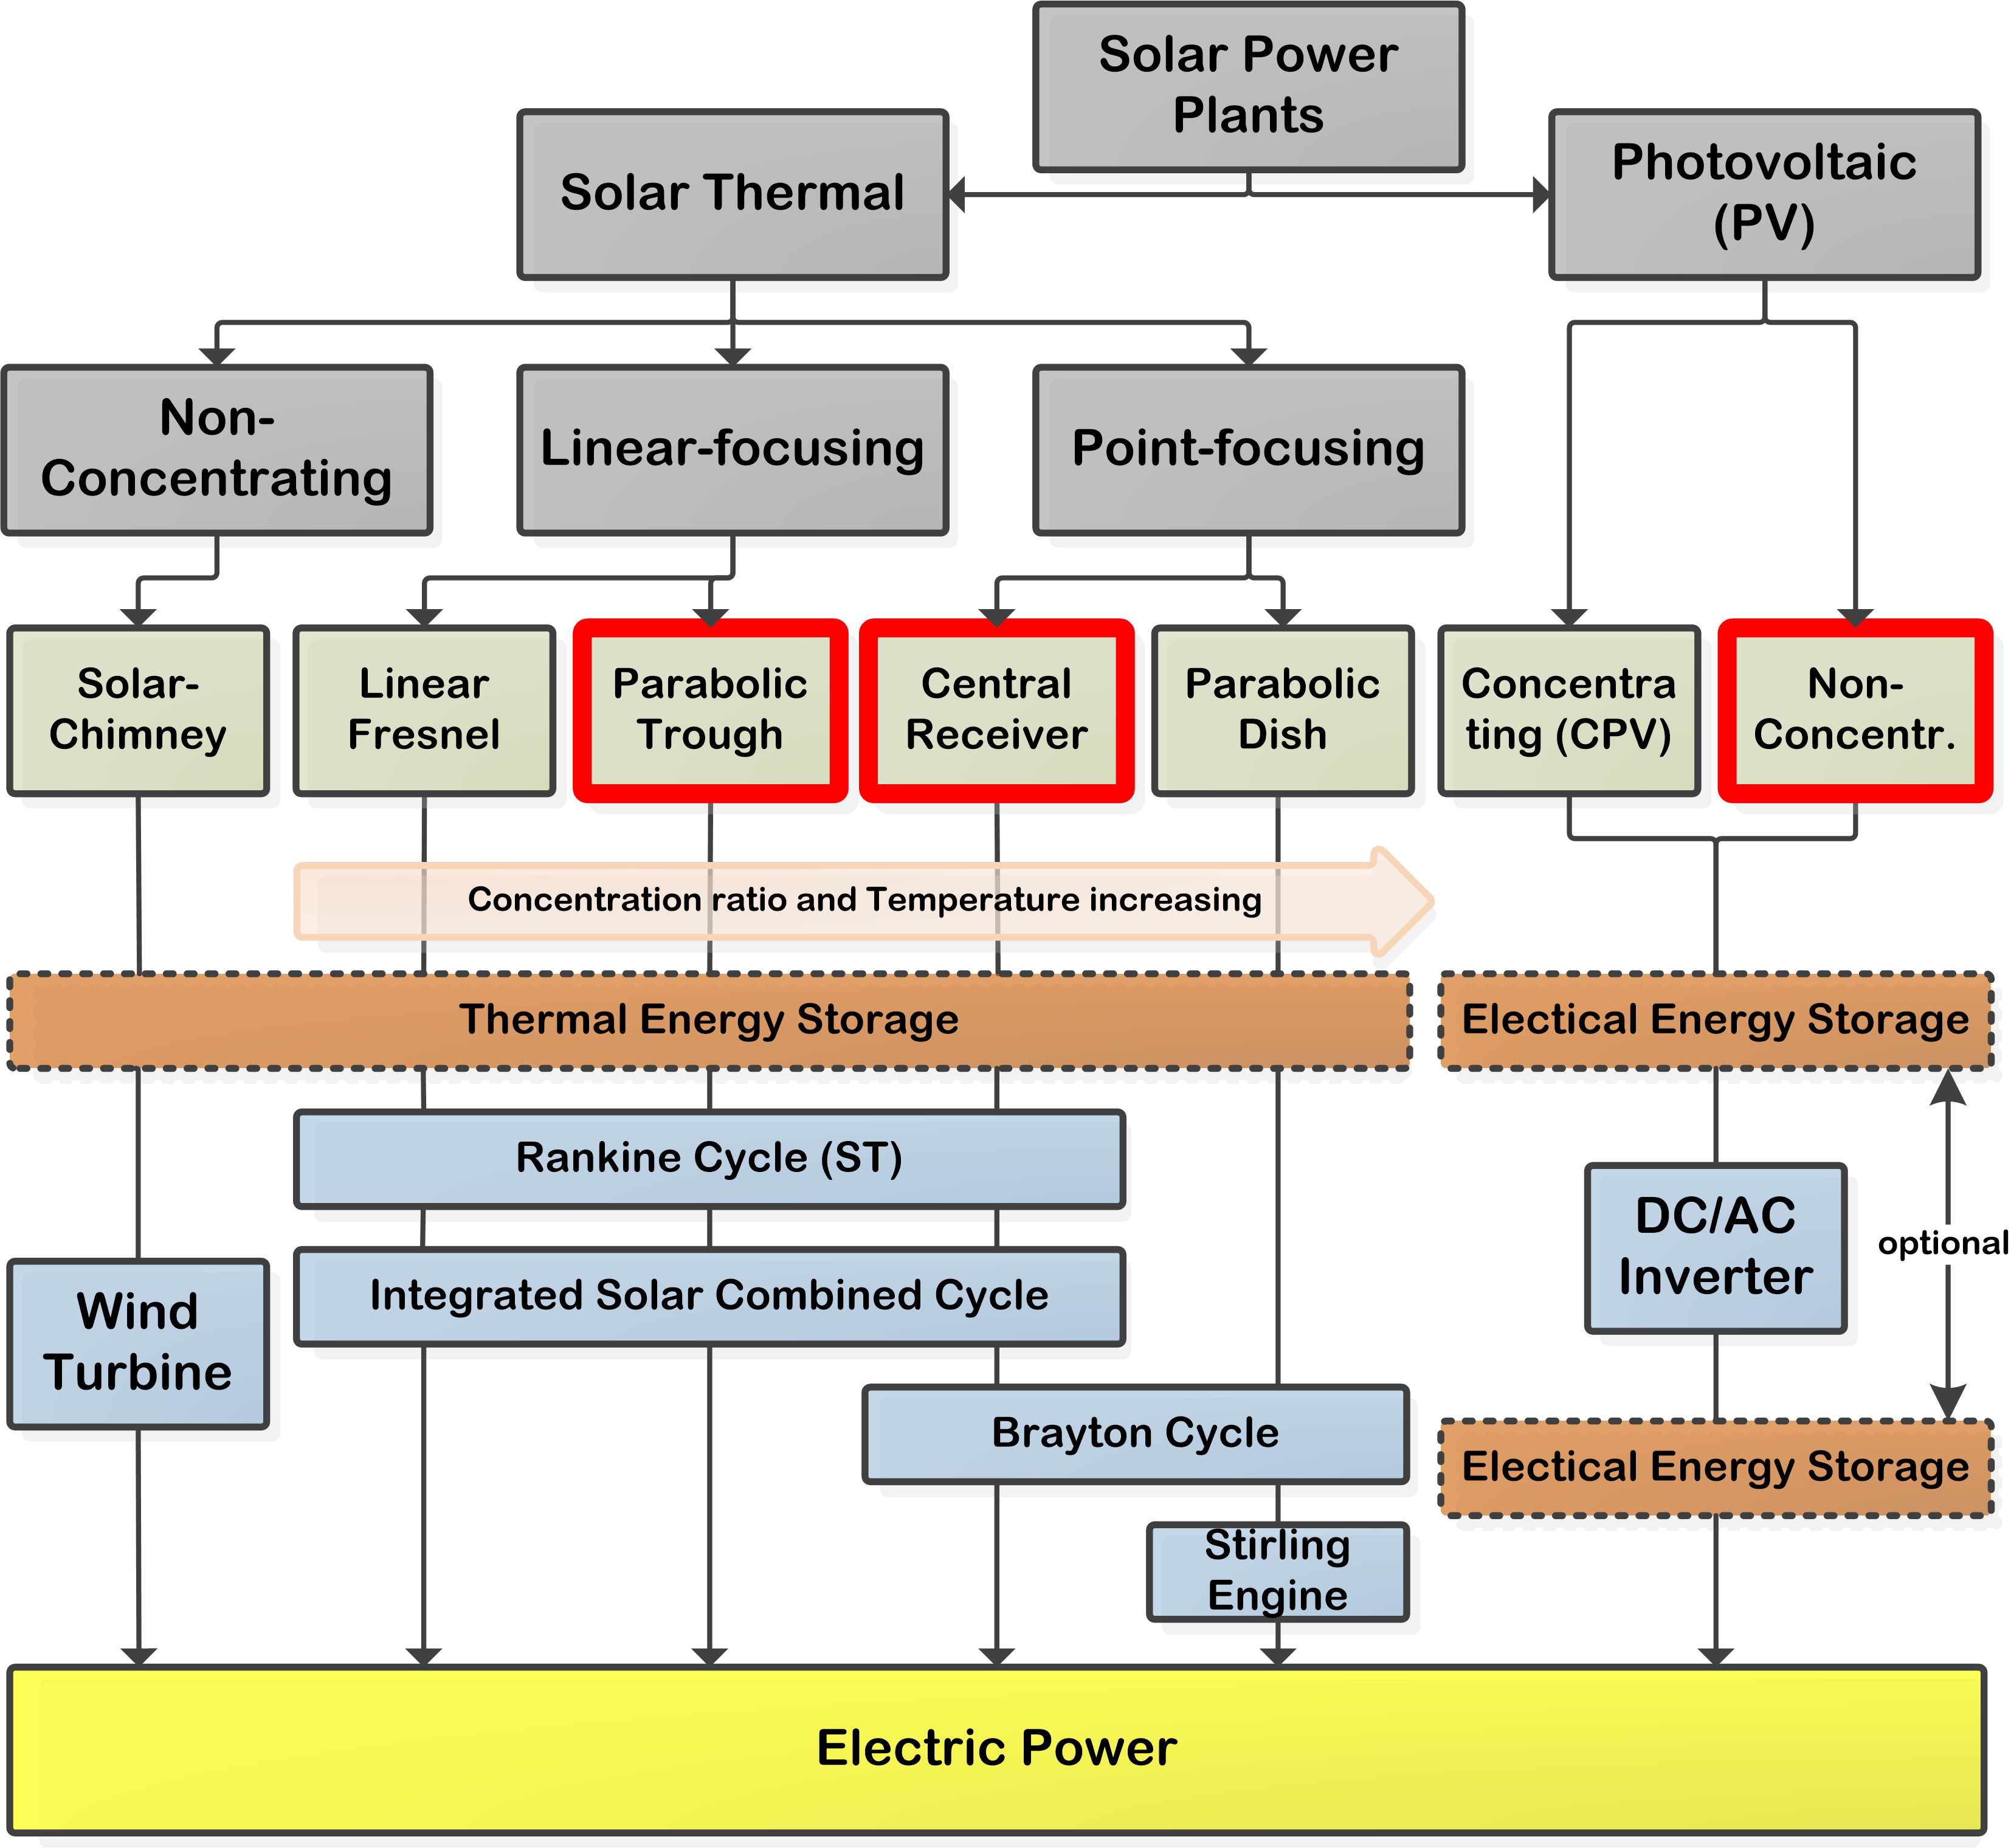
\includegraphics[width=0.75\linewidth]{FIG/OverviewSTP}
\caption[Overview of Solar Power Technologies.]{Overview of Solar Power Technologies.}\label{OverviewSTP}
\end{figure}


Therefore it is split in the technology fields of large scale concentrated solar power plants (\ref{Large scale concentrated solar power (CSP) plants}) and large scale photo voltaic power plants (\ref{Large scale photo voltaic (PV) power plants}).
In detail the technologies with a large-scale power plant potential -- parabolic trough, central receiver and non-concentrating photovoltaic -- are described. Also the storage systems for both systems. 

\section{Large-scale CSP plants}\label{Large scale concentrated solar power (CSP) plants}
Concentrating solar power (CSP) systems use combinations of mirrors or lenses to concentrate direct beam solar radiation to produce forms of useful energy such as heat, electricity and others. This happens by use of various downstream technologies. Generally the CSP technology includes not only the concentrating solar thermal (CST) technology, but also concentrating photovoltaic (CPV) energy conversion. However, there is no focus on CPV in this thesis. That is why the term CST is put on a level with CSP.

A CSP plant comprises four main sub-systems: concentrating system, solar receiver, storage and power block. Also supplementary firing is used in some cases, but is basically not necessary nowadays. A graphic scheme of such a sub-system is shown in Figure~\ref{MainComp}. The separate components are linked together by energy flow in mostly radiation transfer or fluid transport. This chapter describes the function and gives an application overview of the individually components. 
\begin{figure}[!h] 
\centering
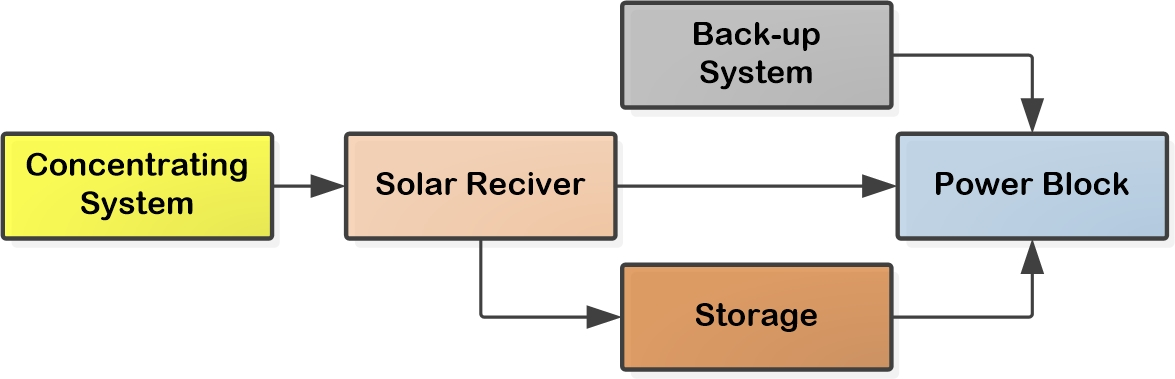
\includegraphics[width=0.85\linewidth]{FIG/MainComp}
\caption[Main components of a CSP plant.]{Main components of a CSP plant.}\label{MainComp}
\end{figure}


The main advantage of CSP in opposite to other renewable energy producers is the thermal storage to provide power for cloudy days or during night time. Therefore the concentrating system and solar receiver have to produce more thermal energy then the power block can use directly. The ratio of the power capacity of the collector field to the capacity of the power block is defined as Solar multiple (SM). For CSP systems with storage, the number of hours of storage is based on the capacity of the power block. Chapter \ref{Subsection_storage_system} describes technical possibilities and application of thermal storage system for CSP.



The solar receiver or concentrating system is eponymously for the main CST technologies. The two most common CSP plant technologies are parabolic trough collector (PTC) and central receiver (CR) systems (also known as solar power towers). Further types of CSP plant are linear Fresnel reflectors (LFR) and parabolic dish. The main difference of the technologies is the concentrating system. Thereof results the differences in optical design, shape of receiver, nature of the transfer fluid and capability to store heat before it is turned into electricity. In systems with a line focus (PTC trough and LFR) the mirrors track the sun along one axis. In those with a point focus (CR and parabolic dish), the mirrors track the sun along two axes. The receiver may be fixed, as in LFR and CR, or mobile as in PTC and parabolic dish systems. An overview of the technologies and there differences in relation to the focus and the receiver  is shown in Table \ref{tbl: CSPtech}.
\begin{table}[h!] % Main technologies 
  \centering
  \begin{tabular}{  m{5cm}  m{5cm}  m{5cm}  }
    \hline
    & \textbf{Line focus} & \textbf{Point focus} \\ 
    & Collectors track the sun along a single axis and focus irradiance on a linear receiver. This makes tracking the sun simpler. & Collectors track the sun along two axes and focus irradiance at a single point receiver. This allows for good receiver efficiency at higher temperatures.\\ \hline \hline
    \textbf{Fixed receiver} & &\\

    Fixed receivers are stationary devices that remain independent of the plant’s focusing device. This eases the transport of collected heat to the power block.
    &
    \begin{minipage}[t]{5cm}
      \centering
	 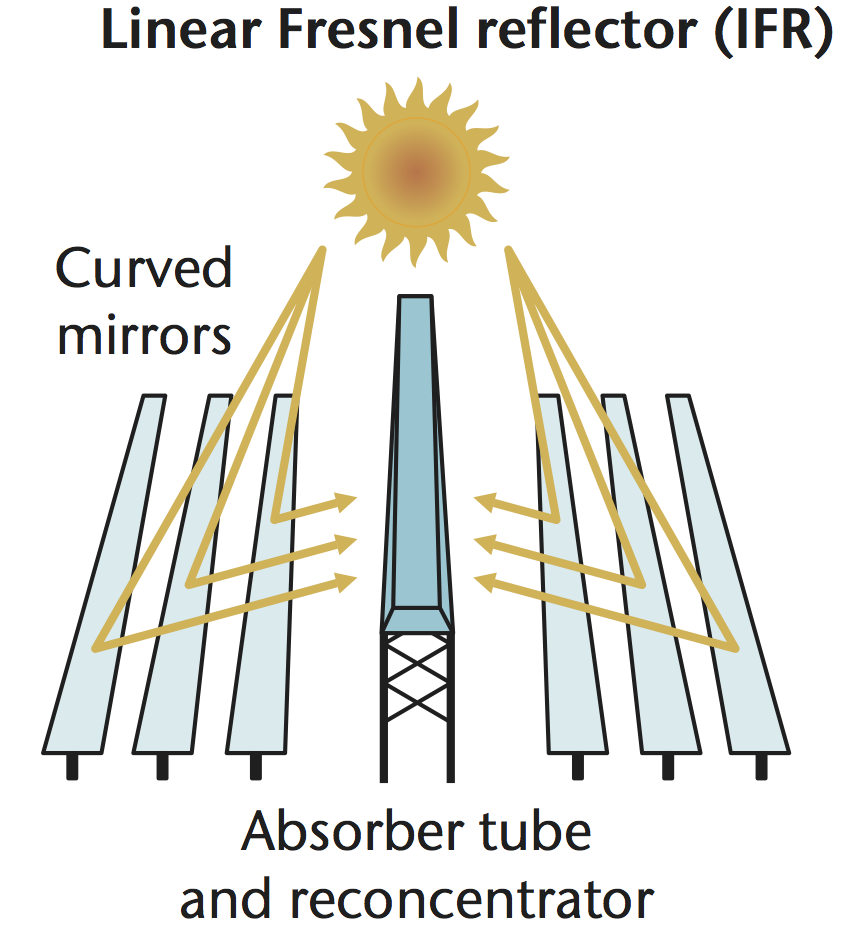
\includegraphics[height=55mm]{FIG/SUM/LF}
    \end{minipage}
    & 
    \begin{minipage}[t]{5cm}
      \centering
	  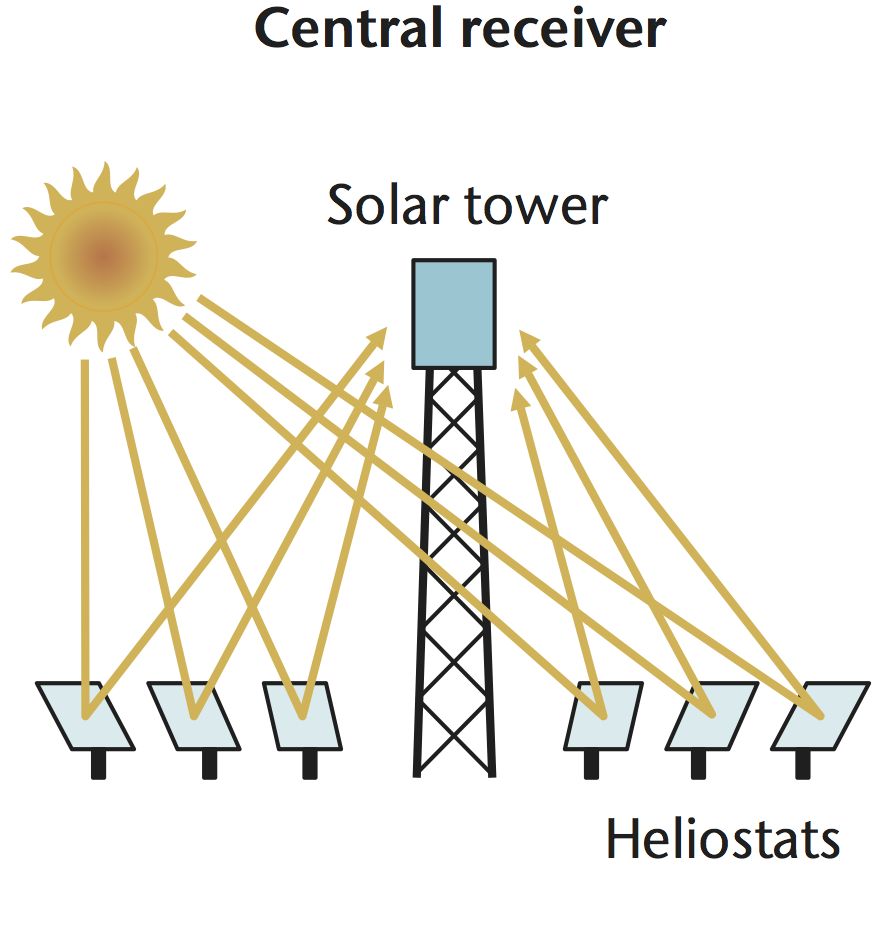
\includegraphics[height=55mm]{FIG/SUM/ST}
    \end{minipage}
    \\ \hline
    \textbf{Mobile receiver} & & \\
    Mobile receivers move together with the focusing device. In both line focus and point focus designs, mobile receivers collect more energy.
    &
    \begin{minipage}{5cm}
      \centering
	  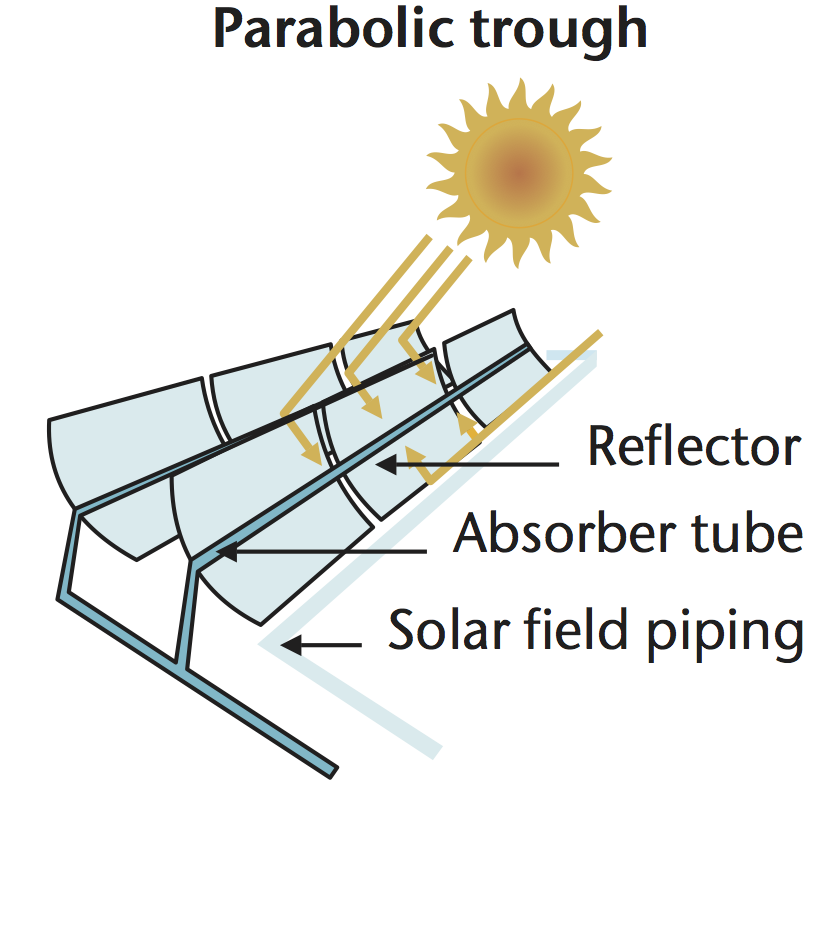
\includegraphics[height=55mm]{FIG/SUM/PT}
    \end{minipage}
    & 
    \begin{minipage}{5cm}
      \centering
	  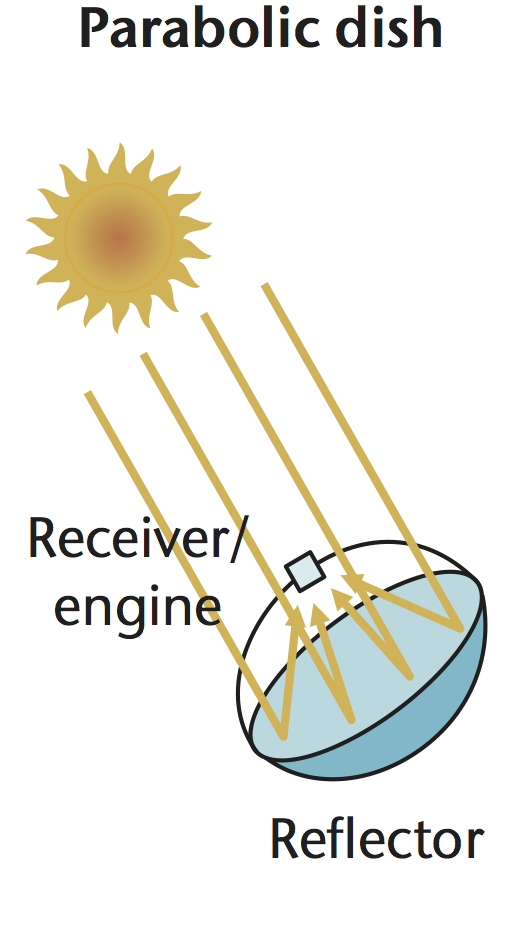
\includegraphics[height=55mm]{FIG/SUM/PD}
    \end{minipage}    
    \\ \hline
  \end{tabular}
  \caption[The main CSP technologies families.]{The main CSP technologies families \cite{IEA2014b}.}\label{tbl: CSPtech}
\end{table}


As mentioned above is main difference between the CSP technology families how they concentrate the solar radiation. This strongly affects their overall efficiency. The parabolic dish has the best annual optical efficiency (about 90\%) because the concentrator axis is always parallel to the sun rays. The worst (about 50\%) is observed for linear Fresnel systems because of poor performance in the morning and in the evening. Intermediate values (65-75\%) are obtained for parabolic trough and tower systems. For each family the actual efficiency varies with the location, the time of day and the season of the year. \cite{EASAC2011} 



The capacity range of an CSP-plant is also strongly affected by the concentration ratio. The most common definition of concentration ratio is the ratio of the area of reflector aperture ($A_a$) to the area of receiver ($A_r$). The area concentration is:
\begin{align}
C=\frac{A_{a}}{A_{r}} \label{GL_concentration}
\end{align}
The concentration ratio from Equation \ref{GL_concentration} has an upper limit that depends on whether the concentration is a three dimensional (point focus) concentrator such as a parabolic dish and central receiver solar tower or a two-dimensional (linear focus) concentrator such as parabolic trough and linear Fresnel reflector. The maximum concentration ratio is based on the second law of thermodynamics applied to radiative heat exchange between the sun and the receiver. The maximum possible concentration ratio for circular concentrators is 45~000, and for linear concentrators is the maximum 212. \cite{Duffie2013}
\begin{table}[h!]  
  \centering
	\begin{tabular}{  p{3.0cm}  C{2.0cm}  C{2.2cm}  C{2.0cm}  C{2.0cm}  C{2.0cm}} 
\hline
\textbf{Technology} & \textbf{Capacity range} $(MW)$ & \textbf{Concent- ration} & \textbf{Peak system efficiency} $(\%)$ & \textbf{Annual system efficiency} $(\%)$ & \textbf{Thermal cycle efficiency} $(\%)$  \\ \hline \hline

Parabolic trough & 10-280$^1$ & 70-100 & 21 & 10-16 & 35-42 ST  \\ \hline
Fresnel reflector & 10-200 & 25-100 & 20 & 9-13 & 30-42 ST  \\ \hline
Solar tower & 10-200 &  300-1~000 & 23 & 8-23 & 0-45 ST  \\ \hline
Dish-Stirling & 0.01-0.4 & 1~000-3~000 & 29 & 16-28 & 30-40  \\ \hline
\multicolumn{2}{l}{ST = Steam Turbine}
\end{tabular}
\caption[Performance Characteristics of main CSP technologies families.]{Performance Characteristics of main CSP technologies families \cite{Pitz-Paal.2013} \cite{AbengoaSolar2013a}$^1$.}\label{tbl: CSPCharacteristics}
\end{table}


But actually the technical implementation of concentration ratio is the main parameter for the capacity range of a CSP plant. Table~\ref{tbl: CSPCharacteristics} gives an overview of some of the performance characteristics of the concentrating solar power concepts. More details are listed in Annexure I, Part A, Figure~\ref{CSPOverview1} on Page~\pageref{CSPOverview1} and Figure~\ref{CSPOverview2} on Page~\pageref{CSPOverview2}. PTC, LFR, and CR can be coupled to steam cycles of 10-280~MW electric capacity (and more), with thermal cycle efficiencies of 30-45~\%. Also the applies for stirling engines which are coupled to dish systems have similar efficiency ranges. The conversion efficiency of the power block remains essentially the same as in conventional-fired power plants. The annual system efficiency are the net power generation over incident beam radiation. They are lower than the conversion efficiencies of conventional steam or combined cycles, because they include the conversion of solar radiative energy to heat within the collector and the conversion of the heat to electricity in the power block. \cite{Pitz-Paal.2013}

\begin{figure}[!h] 
\centering
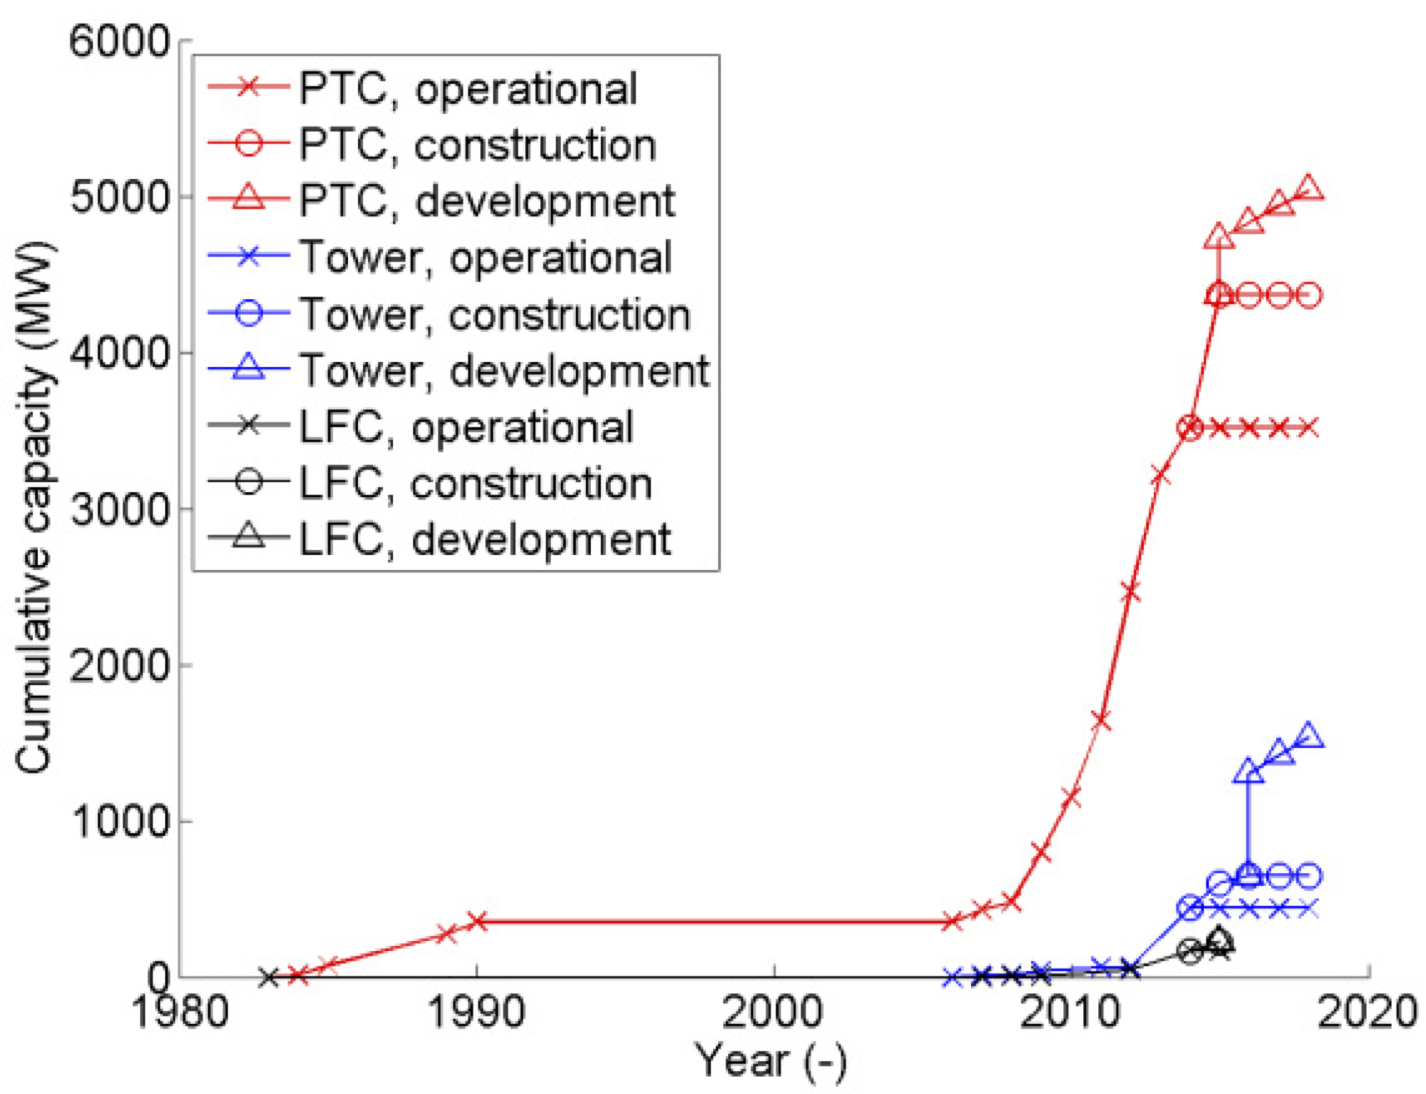
\includegraphics[width=0.65\linewidth]{FIG/CSP_technology_development}
\caption[Historical development of CSP technologies.]{Historical development of CSP technologies \cite{Abbas2015}.}\label{CSP_technology_development}
\end{figure}

The development of the actual CSP plant technology goes back in the 1970's and 1980's, which is a consequent from the first two Oil crises. Figure~\ref{CSP_technology_development} shows the historical development of PTC, LFR in the Figure called linear Fresnel collector (LFC) and the CR (tower). The parabolic dishes have not succeeded at all and aren't shown here. The reason for that is mainly due to the high structural costs of moving an large diameter dish with two-axes tracking. One might observe that the predominant technology is the PTC, with an installed capacity well above 3~GW. CR have started the exponential development some years later compared to PTC, which explains why the operational installed capacity is much lower. Similarly the development for LFR have started even later, which drives to the lowest installed capacity of the three technologies. The difference in the timing of the three successful technologies is very influenced by the CSP development in its first golden period, the 1980's. In such period important central tower prototypes were built in USA (Solar One, Solar Two, CESA-1) and a 365~MW PTC solar plant was installed in the Mojave Desert. When the oil prices dropped at the end of the second oil crises interest on renewable energies was lost until the last decade. 



With regard to the past development in the different CSP technology dealt the following chapters with the PTC (\ref{subsection_PTC}) as well as with the solar tower technology (\ref{subsection_CRS}). The necessary concepts of the storage systems (\ref{Subsection_storage_system}) and an overview of common heat transfer fluids (\ref{subsection_HTF}) are also included. The systems for the converting thermal to electrical power will be also summarized (\ref{subsection_powerblock}).  Parabolic dishes and LFC are not further considered depending to the development stage.
\pagebreak
\subsection{Parabolic-trough concentrating solar power} \label{subsection_PTC}
Parabolic trough power plants consist of many parabolic-trough-shaped concentrator that reflects direct solar radiation onto a receiver or absorber tube (also called receiver tube) located in the focal line of the parabola. The heated fluid is used in a steam generation system, to drive a steam turbine/generator cycle. Optional thermal storage and/or fossil-fired backup systems are possible. A schematic concept of a parabolic trough power plant is shown in Figure \ref{parabolic_troughs}. The collector field is made up of a large number of single-axis-tracking parabolic trough solar collectors and receivers. The solar field is modular in nature and comprises many parallel rows of solar collectors, normally aligned on a north-south horizontal axis. The collectors track the sun from east to west during the day to ensure that the sun is continuously focused on the linear absorber tube.
\begin{figure}[!h] 
\centering
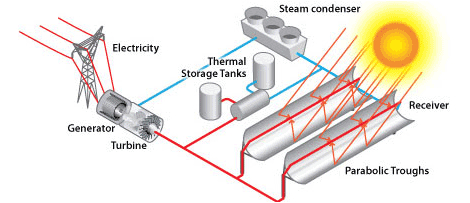
\includegraphics[width=0.7\linewidth]{FIG/parabolic_troughs}
\caption[Schematic parabolic trough power plant concept.]{Schematic parabolic trough power plant concept \cite{U.S.DOE2013}.}\label{parabolic_troughs}
\end{figure}


The first graphically documented parabolic-trough solar collector was designed and built in 1870 by Swedish engineer John Ericsson. This collector produced 373~W by a steam engine had and had a solar radiation collecting surface of 3.25~m$^2$. \cite{Fernandez-Garcia2010}

Current PTC are based on developments in the united states which began after the first oil crisis. In the 1980s the first commercial used PTC plants was build. Most outstanding the implementation of the nine SEGS (Solar Electricity Generating System) plants. Build from 1984 (SEGS-I) to 1990 (SEGS-IX) in the Mohave Desert (California, USA) by LUZ International Limited and still operating. In total they have an electrical output of 354 MW and more than two million square meters of parabolic-trough collectors. They using oil to produce steam in heat exchangers before being circulated back to the solar field. Like in a electricity generating plant the steam is used in a conventional steam turbine. After the cutting down of government incentives for renewable systems and the oil price fell again in the 1980s the installation of more SEGS plants went unfeasible. \cite{Kalogirou2014a}

But the technology is still applied in most of the present build commercial parabolic trough power plants. Today they are using as HTF synthetic oil, typically out of biphenyl/diphenyl oxide fluid. The maximum cycle temperature is limited to values below 400$\,^{\circ}\mathrm{C}$ in order to avoid decomposition of the HTF. The thermal energy from the solar field is transported by the HTF to the heat-exchanger steam generator systems providing the superheated steam for the turbine of typically 370-380$\,^{\circ}\mathrm{C}$. The limitation of the upper process temperature to about 400$\,^{\circ}\mathrm{C}$ can be overcome by changing the HTF. A higher process temperature leads to a significant increase in the thermodynamic conversion cycle efficiency. A summary of current applied HTFs can be found in Chapter~\ref{subsection_HTF}.

An alternative HTF is water/steam, which is used in the steam cycle any way. The direct steam generation (DSG) in parabolic trough collectors demonstration loops steam reaches temperature of 550$\,^{\circ}\mathrm{C}$. Aside from the process temperature, the benefits of DSG compared with oil are based on savings in the heat exchanger, in reduced pumping effort, and the uncritical handing of the medium. But there are still barriers for commercial scale application. Some of the most important technological challenges of the DSG parabolic trough plant are the control stability, receiver tube viability, and collector interconnection feasibility.  \cite{Alguacil2014}

Another alternative HTF for PTC is molten salt. Salts already proved there competence in solar tower power plants and also application of liquid salts in parabolic trough systems have been investigated. Salts has suitable thermophysical properties, namely high boiling and decomposition point, low vapor pressure, high specific heat capacity, high thermal conductivity, and high density at low pressures \cite{Cordaro2011}. Molten salt has also the advantage to be the art of science in thermal storage for large- scale CSP plants (see Chapter \ref{Subsection_storage_system}).  Furthermore, typical salt mixtures are significantly cheaper than synthetic oils \cite{Gil2010}. The 5~MW Archimede commercial PTC plant is using a mixture of sodium nitrate (60\%) and potassium (40\%) nitrate since 2010 \cite{NREL2012}. The upper solar-field outlet temperature is 550$\,^{\circ}\mathrm{C}$ but starts crystallization of the non-eutectic melt occurs at 238$\,^{\circ}\mathrm{C}$ \cite{Cordaro2011}. That is one concerns with molten salt-based parabolic trough plants. The solar plant needs to be fully equipped with impedance and trace heating systems in order to ensure non-freezing of the salt. Therefore also the the process setup needs to be modified. But according to the researcher of the "Archimede Solar Energy molten salt parabolic trough demo plant" the molten salt parabolic trough (MSPT) technology is mature for large scale commercial applications without any critical points to be addressed \cite{Maccari2015}. Also the higher investment costs in solar field and piping, as well as maintenance and operation cost seams to be manageable and will be overcome to the increase in total plant efficiency and lower storage and HTF costs. Therefore the expected levelized cost of electricity (LCoE) of PTC power plants will decrease around 20\% \cite{Richert2015}. Component manufacturers are starting to introduce products specifically aimed at this technology. Upcoming projects needs to validate this expected decrease of LCoE in commercial scale and represent their profitability. \\ 


As mentioned above a PTC power plant consists out of the components collector and receiver, which held together by support structure. This components are connected in loops, which building the solar field.
\subsubsection{Parabolic Trough Collectors}
The task of PTC module is to reflect the radiation of the sun accurately to the receiver tube. So the main components of a PTC module are actually the curved mirror and the absorber tube. But usually the PTC means the reflector and its support structure. The absorber tubes are separately regarded. The structure holds the components in place and connects the reflector modules between each other. To concentrate the radiation to the absorber tube the shape of the reflective surface is in parabolic form like in Figure \ref{PTC_section}. There shown is a section of a PTC with the dimensions of the commercial used LS-3, EuroTrough and Senertrough-1 and their focus point. This focus point is only at this position when the z-axis is in the direction of the Sun. Therefor the PTC is controlled by means of astronomical calculations, often supplemented by a Sun position sensor. The absorber tubes mounted in the focal line move with the collector and are connected to the stationary field piping via flexible hoses or rotating joint arrangements.
\begin{figure}[!h] 
\centering
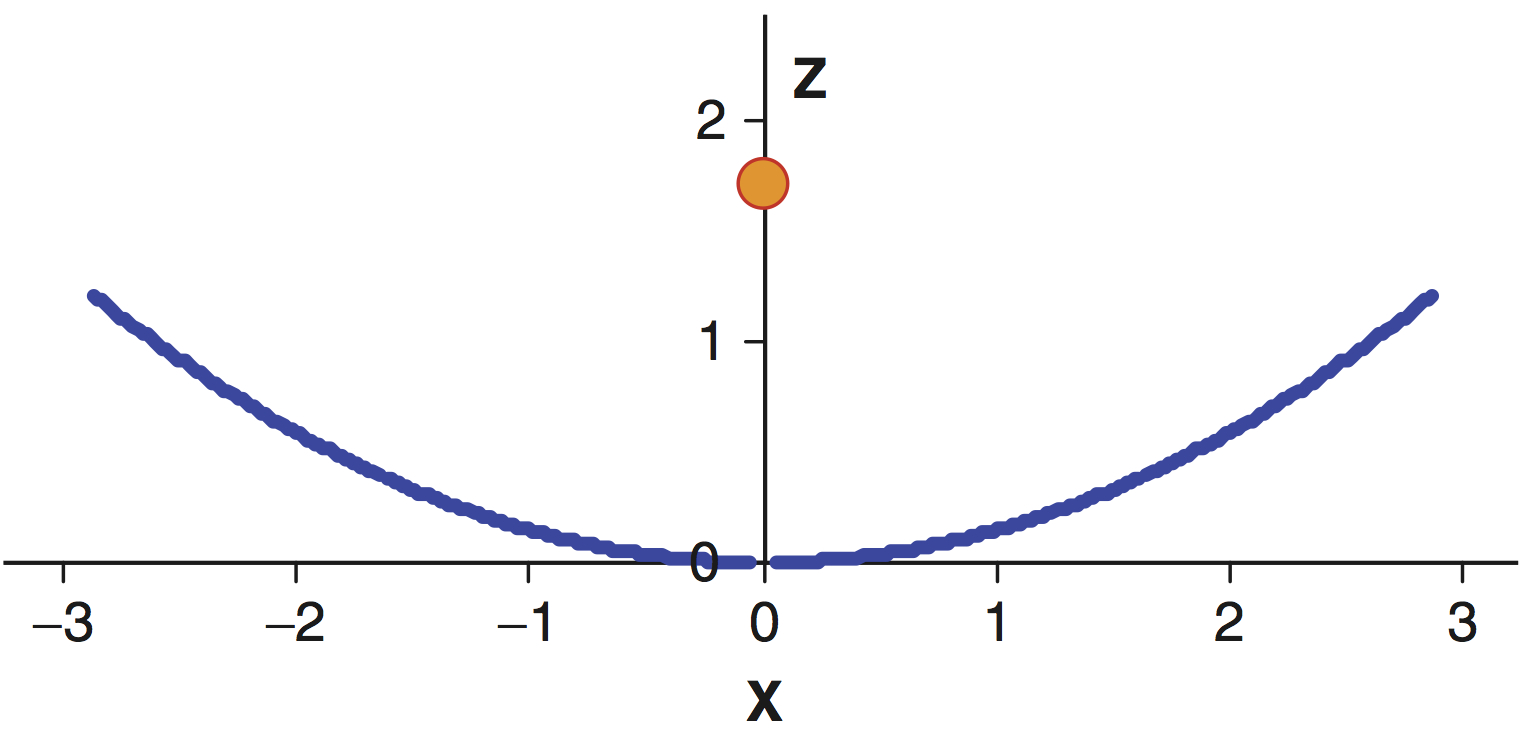
\includegraphics[width=0.6\linewidth]{FIG/PTC_section}
\caption[PTC section – dimensions of EuroTrough, LS-3, and other designs, in meters.]{PTC section – dimensions of EuroTrough, LS-3, and other designs, in meters \cite{Lupfert2013}.}\label{PTC_section}
\end{figure}


The history of PTC goes far back to 1870, where they already used small engines with solar power \cite{Fernandez-Garcia2010}. With the time of the first oil crisis in the 1980s also new PTC were developed. In this decade also the collector family LS-1, LS-2 and LS-3 was developed by LUZ. These PCT  were implement in the first large-scale solar thermal power plants SEGS 1 (1984) to SEGS 9 (1990) in California. The used PTC features a modular design based on steel structures with parabolic preshaped, silvered glass mirrors and improved efficiency by implementation of evacuated tube receivers. A European consortium designed in the late 1990s the EuroTrough. Which was based on the LS-3 concentrator geometry with a focal length (the shortest distance from the mirror to the focal line) of 1.71~m and an aperture (the projection of the concentrator area in the direction of the optical axis) width of 5.77~m, but offered advantages in stiffness and costs \cite{Osuna2001}. Some years later, SENER developed a different structural approach, but still maintained the basics of LS-3 concentrator geometry \cite{Fernandez-Garcia2010}.
\begin{figure}[!h] 
\centering
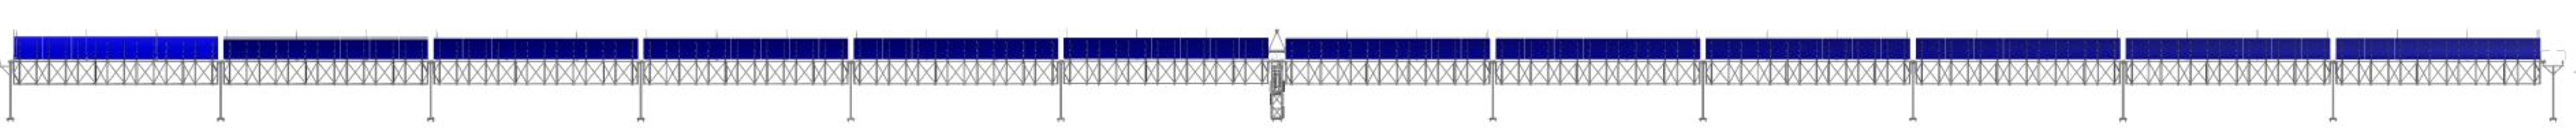
\includegraphics[width=1\linewidth]{FIG/SCA_EuroTrough}
\caption[Solar Collector Assembly (SCA) composed of 12 EuroTrough collector elements (SCE).]{Solar Collector Assembly (SCA) composed of 12 EuroTrough collector elements (SCE) \cite{VonReeken2014}.}\label{SCA_EuroTrough}
\end{figure}


PTC are typically assembled from solar collector element (SCE), mounted on a series of aligned pylons. The center pylon is equipped with a hydraulic drive system to allow tracking of the total solar collector assembly (SCA). Figure~\ref{SCA_EuroTrough} shows the SCA of the EuroTrough. From 12 SCE of the SCA results a total length of approximately 150~m and 816~m$^2$ \cite{VonReeken2014}. 

Table \ref{tbl: TroughCharacteristics} illustrates that recent developments show a continuing trend towards larger aperture sizes such as for the Heliotrough, Senertrough-2 and Ultimate Trough. The development steps of the aperture size are exemplary shown in Figure \ref{Kollektoren} for EuroTrough, Heliotrough and Ultimate-Trough. 

\begin{table}[h!]  
  \centering
	\begin{tabular}{  p{3.3cm}  C{1.0cm}  C{1.0cm}  C{1.5cm}  C{1.0cm}  C{1.0cm}  C{1.0cm}  C{1.0cm}  C{1.5cm}} 
\hline
\textbf{Property} & \textbf{LS-1} & \textbf{LS-2} & \textbf{LS-3} & \textbf{Euro-Trough} & \textbf{Helio-trough} & \textbf{Sener-trough-1} & \textbf{Sener-trough-2} & \textbf{Ultimate-Trough} \\ \hline \hline
Start of development & 1984 & 1985 & 1989 & 1998 & 2005 & 2005 & 2006 & 2009 \\ \hline
Aperture width [m] & 2.55 & 5.00 & 5.77 & 5.77 & 6.78 & 5.77 & 6.87 & 7.51 \\ \hline
Length per module/SCE [m] & 6.3 & 8 & 12 & 12 & 19 & 12.27 & 13.23 & 24 \\ \hline
SCA length [m] & 50.2 & 47.1 & 99 & 147.8 & 191 & n.a. & 158.8 & 242.2 \\ \hline
Focal length [m] & 0.68 & 1.40 & 1.71 & 1.71 & 1.71 & 1.71 & 2 & n.a. \\ \hline
\end{tabular}
\caption[Characteristics of different parabolic trough collectors.]{Characteristics of different parabolic trough collectors \cite{Pitz-Paal.2013}.}\label{tbl: TroughCharacteristics}
\end{table}


The use of lager collector units with more aperture area brings some advantages. The Ultimate Trough shows a cost reduction of about 20 to 25\% compared to the EuroTrough. Coming from lower specific costs and increased of optical performance. Also the amount of heat transfer fluid can be reduced by 25\%. This promise an decreased LCoE by about 11\% compared to EuroTrough. \cite{VonReeken2014}
\begin{figure}[!h] 
\centering
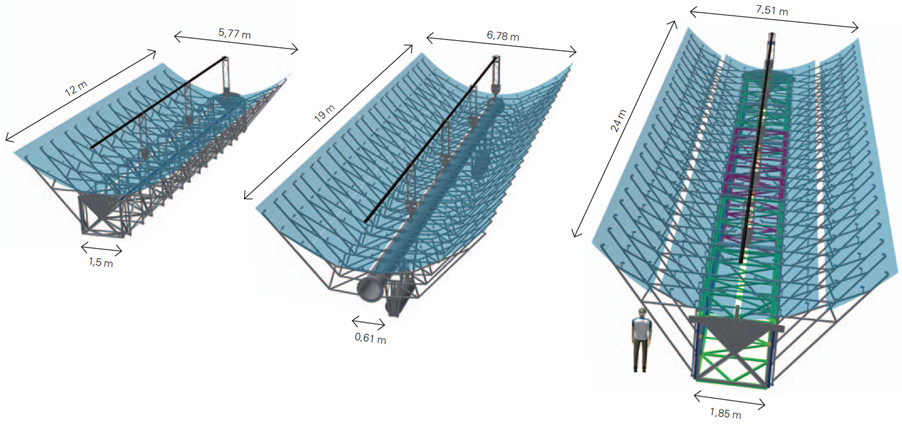
\includegraphics[width=1\linewidth]{FIG/Kollektoren}
\caption[Evolution of parabolic trough collector sizes over 3 development cycles (Eurotrough, HelioTrough, Ultimate Trough).]{Evolution of parabolic trough collector sizes over 3 development cycles (Eurotrough, HelioTrough, Ultimate Trough)\cite{Schlaichbergermannundpartner}.}\label{Kollektoren}
\end{figure}


Another approach to reduce costs is the utilization of other reflector materials. The Skytrough uses reflectors made from silvered polymer film laminated to aluminum sheets mounted on a space frame. Compared the to the costs of components of the EuroTrough, the Skytrough contribute an additional 34\% cost savings in combination with a aperture width of 6.0~m \cite{Mason2014}. Thin glass on a glass-fiber/foam sandwich was used for the SL4600 construction \cite{SolarliteCSPTechnologyGmbH2014}. Both approaches take advantage of the mechanical strength of the mirrors to reduce the amount of additional steel structure required.

Abengoa Solar is developing currently the "SpaceTube" concept, using 8~m aperture width and will use 80~mm diameter absorber tubes. \cite{Olar2013}
\pagebreak
\subsubsection{Absorber tube (Receiver)}
The absorber tube or also called receiver is the component where solar energy is converted to thermal energy in the form of sensible or latent heat of the fluid that circulates through it. This component produces the predominant share of thermal losses in an parabolic trough power plant, for that reason it is also one of the most critical and important performance components \cite{Lupfert2013}. Currently, there are just two types of receiver for parabolic trough power plants, classified as either evacuated or non-evacuated. Evacuated receivers are commonly used for temperatures above 300$\,^{\circ}\mathrm{C}$ and its consist of three main parts. The metal absorber tube, an protection glass tube and the connection unit with expansion bellows. In order to reduce thermal losses and increasing the overall efficiency of the PTC the receiver unit uses a high vacuum (i.e.,~10-5~mbar) between the metal absorber tube and the protection glass. Figure shows \ref{absorber_tube} the structure of an typical vacuum tube receiver. 
\begin{figure}[!h] 
\centering
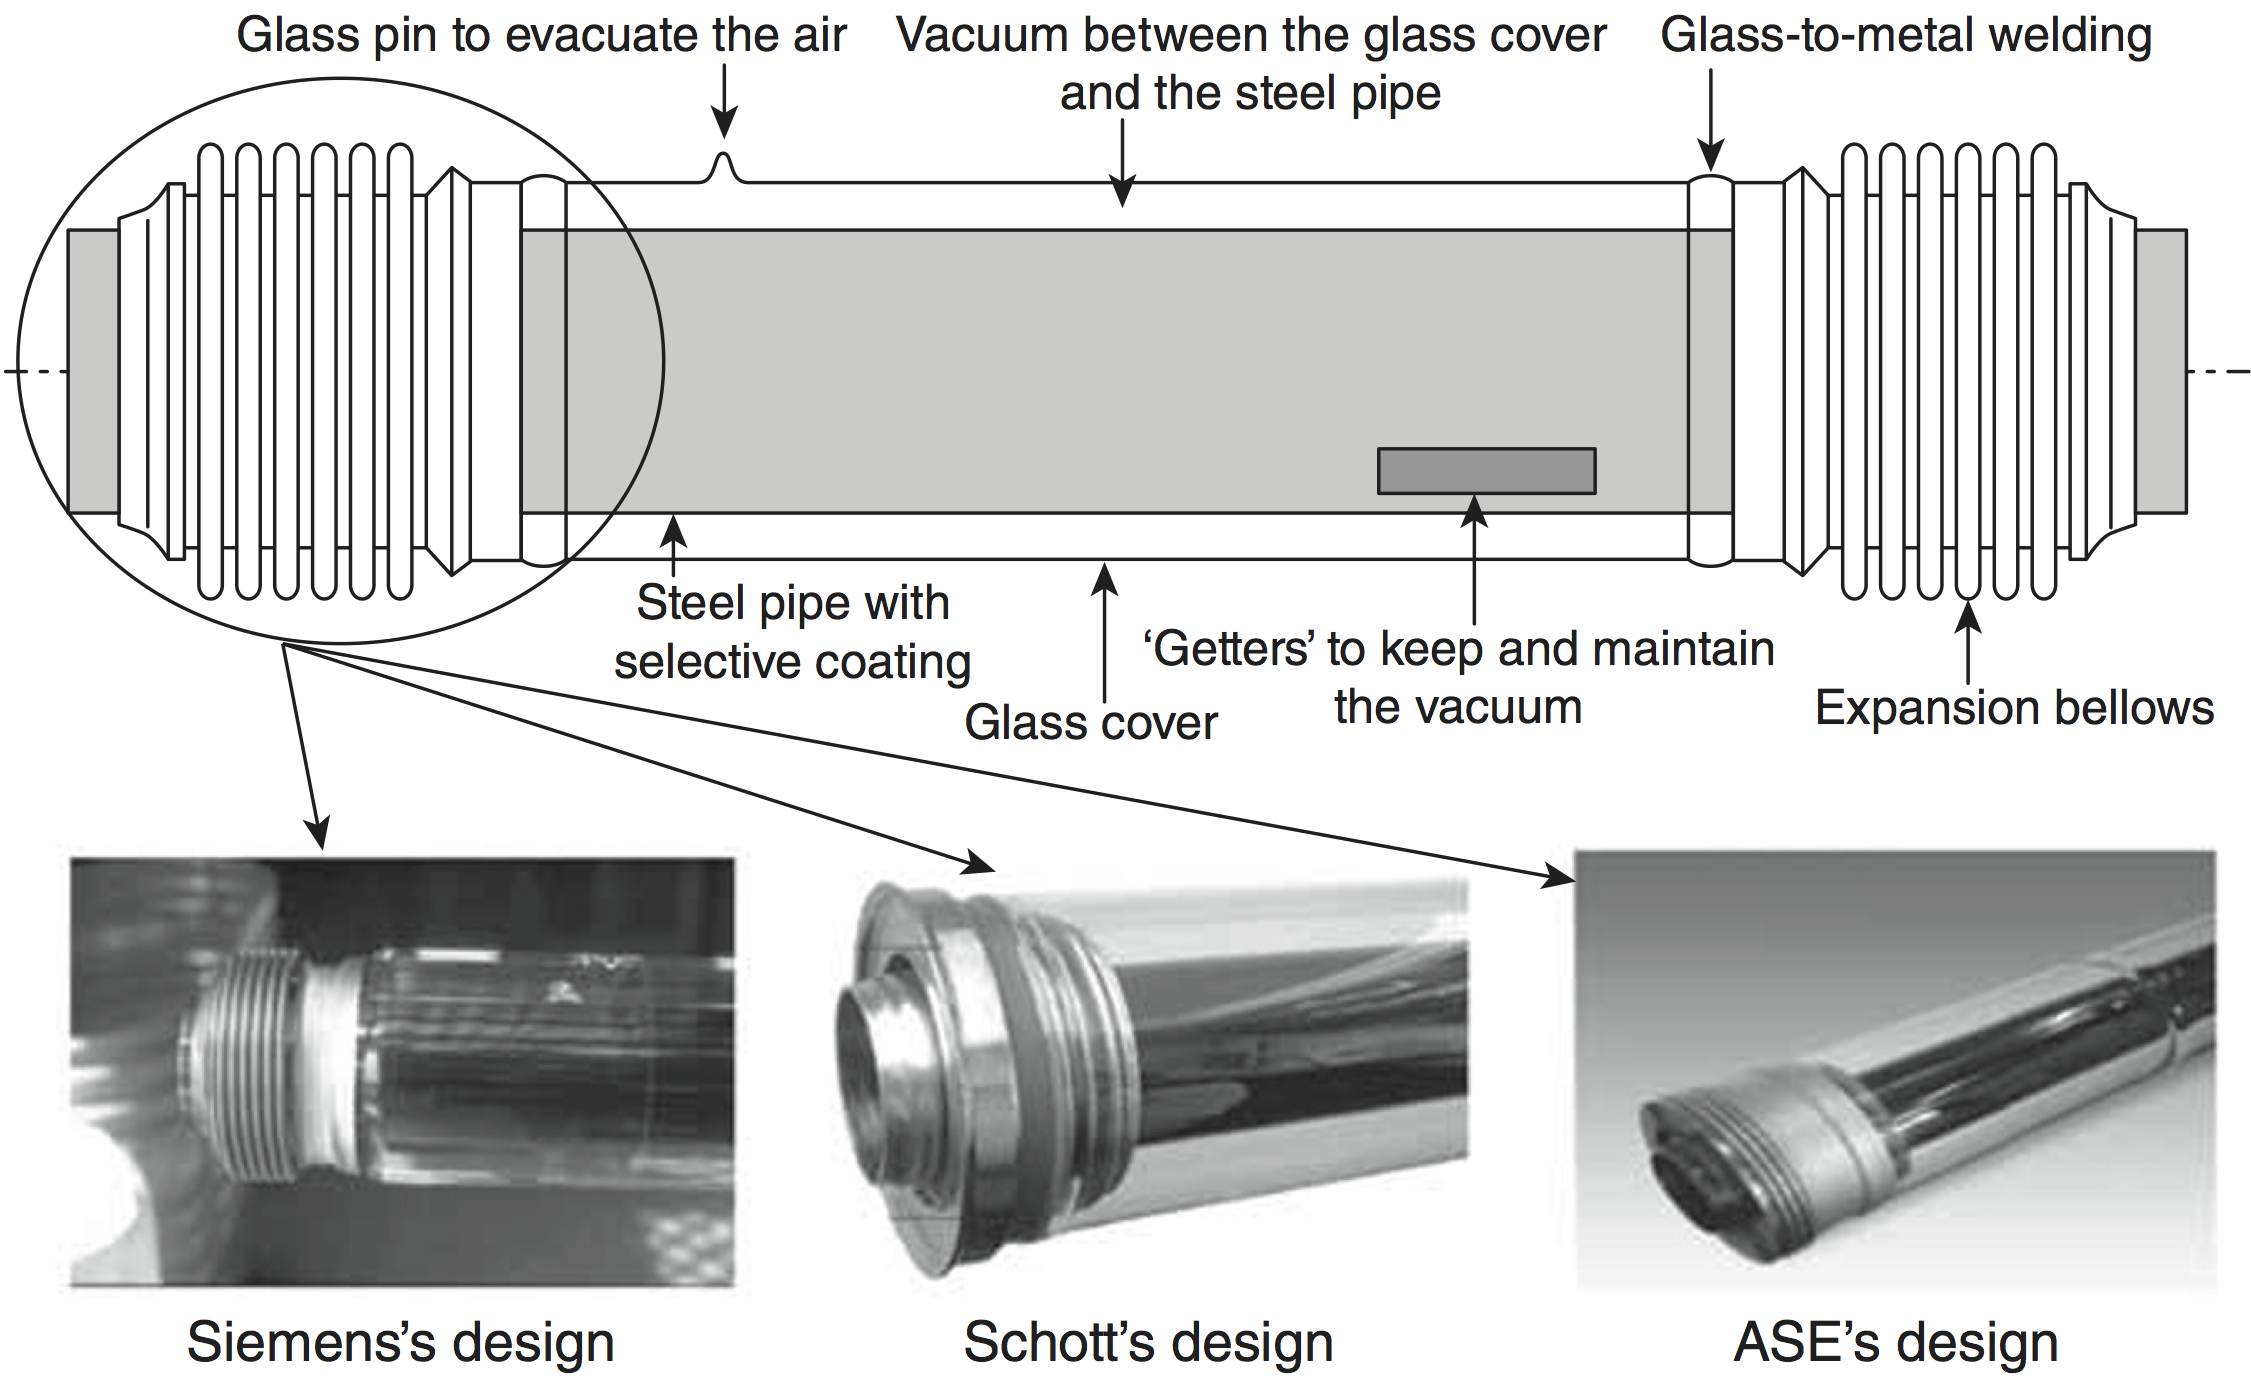
\includegraphics[width=0.9\linewidth]{FIG/absorber_tube}
\caption[A typical evacuated receiver for parabolic-trough collectors.]{A typical evacuated receiver for parabolic-trough collectors \cite{Moya2012}.}\label{absorber_tube}
\end{figure}
\\

The metal absorber tube is a dark-coated to absorb the incoming solar radiation. It absorbs the concentrated radiation reflected from the mirror, and also the global radiation hitting from top. The outer surface of the metal absorber tube has an optically selective surface with a high solar absorptance and low emittance for thermally generated infrared radiation. This is achieved with sputtered Cermet coatings consisting of several layers of metallic and ceramic coatings. Also, galvanic black-nickel and black-chrome coatings are applied but have less temperature resistance and higher emissivity. \cite{Platzer2012}



The protection glass is connected to the metal absorber tube by means of stainless steel expansion bellows. These bellows compensate the thermal expansion of glass and steel which results at nominal working temperature. Therefore one end of these expansion bellows is directly welded to the outer surface of the metal absorber tube, while the other end is connected to the end of the protection glass by means of a glass-to-metal welding. The glass-to-metal welding is a weak point in the absorber system and has to be avoid by high thermal and mechanical stress that could cause the welding to crack. The receiver provider has various solution for the expansions bellows. Figure \ref{absorber_tube} shows also the solutions of three manufacturers (Schott, Siemens and ASE) joining the protection glass and the inner metal absorber tube. The expansion bellows also provide a tight annular gap between both tubes to make the vacuum. To support the shelf life of the vacum chemical ‘getters’ can be placed in the gap between the metal absorber tube and the protection glass to absorb gas molecules.
\begin{table}[!h]  
  \centering
	\begin{tabular}{  p{3.5cm}  C{3.5cm}  C{3.5cm}  C{3.5cm} } 
	
	\hline	
 & \textbf{Schott PTR-70} & \textbf{Siemens UVAC-2010} & \textbf{ASE HEMS08}\\ \hline \hline

Solar absorptance & $\ge$~0.95 & $\ge$~0.96 & $\ge$~0.95 \\ \hline
Solar transmittance & $\ge$~0.96 & $\ge$~0.96 & n.a. \\ \hline
Thermal emittance & $\le$~0.1 at 400$\,^{\circ}\mathrm{C}$  & $\le$~0.9 at 400$\,^{\circ}\mathrm{C}$& $\le$~0.1 at 400$\,^{\circ}\mathrm{C}$  $\le$~0.14 at 580$\,^{\circ}\mathrm{C}$\\ 
Steel pipe inner/ outer diameters & 70/65~mm stainless steel & 70/65~mm stainless steel & 70/65~mm stainless steel \\ \hline
Thermal losses & 250 W/m at 400$\,^{\circ}\mathrm{C}$ & n.a. & 230 W/m at 400$\,^{\circ}\mathrm{C}$ \\ \hline
Glass cover & Borosilicate & Borosilicate & Borosilicate\\ \hline
Active length ratio at 350$\,^{\circ}\mathrm{C}$ & >96\% & 96.4\% & n.a.\\ \hline
Maximum fluid temperature & 400$\,^{\circ}\mathrm{C}$ & 400$\,^{\circ}\mathrm{C}$ & 550$\,^{\circ}\mathrm{C}$\\ \hline
\end{tabular}
\caption[Technical parameters of the receivers commercialized by Schott, Siemens and ASE.]{Technical parameters of the receivers commercialized by Schott, Siemens and ASE \cite{Moya2012}.}\label{tbl: receiver_details}
\end{table}
\\

Most of the parabolic-trough solar thermal power plants implemented around the world until 2009 had receivers manufactured by either the Israeli company, Solel (purchased in 2009 by Siemens and 2013 from Abengoa \cite{Alcauza2013}), or the German company, Schott. In 2009, the Italian company, Archimede Solar Energy (ASE), announced that they were launching a new receiver tube called HEMS08, suitable for fluids up to 550$\,^{\circ}\mathrm{C}$. The first plant using HEMS08 receivers was the Archimede Plant, located in Syracuse (Italy) and ready to operate in 2010 using molten salt as HTF. Most widespread geometry is the receiver, with 70~mm absorber tube diameter, but due to larger aperature width of the trough reflectors, also the absorber tube diameter is raising. The technical details of the receivers manufactured 2012 by Schott, Siemens and ASE are shown in Table \ref{tbl: receiver_details}. Schott's PTR-70 is now in the 4. generation, the actual UVAC 70-7G is now in production by Rioglass a subsidiary from Abengoa Solar and ASE's present molten salt receiver tube is the HCEMS-11, but in generally the technical parameters are still up-to-date \cite{Schott2015,ArchimedeSolarEnergy2015,RioglassSolarInternational2014}.
\\

Most widespread geometry is the receiver, with 70~mm absorber tube diameter, but due to larger aperature width of the trough reflectors, also the absorber tube diameter is raising. This is a further contribution to using molten salt as future HTF in large-scale PTC power plants. 
\pagebreak
\subsubsection{Field}
The heat-collecting portion of the PTC power plant is the solar field. It consists of one or more parallel loops of SCAs. A common header pipe provides each loop with an equal flow rate of HTF. A second header collects the hot HTF to return it either directly to the power cycle for power generation or to the thermal energy storage system for use at a later time. To minimize pumping pressure losses, the field is typically divided into multiple sections, each section with its own header set, and the power cycle is situated near the middle of the field. The size of the field depends on required thermal power for the power block and the storage system. The orientation of the field depends obviously on the orientation of the parabolic collectors, which are installed with their north-south oriented rotation axis.
\begin{figure}[!h] 
\centering
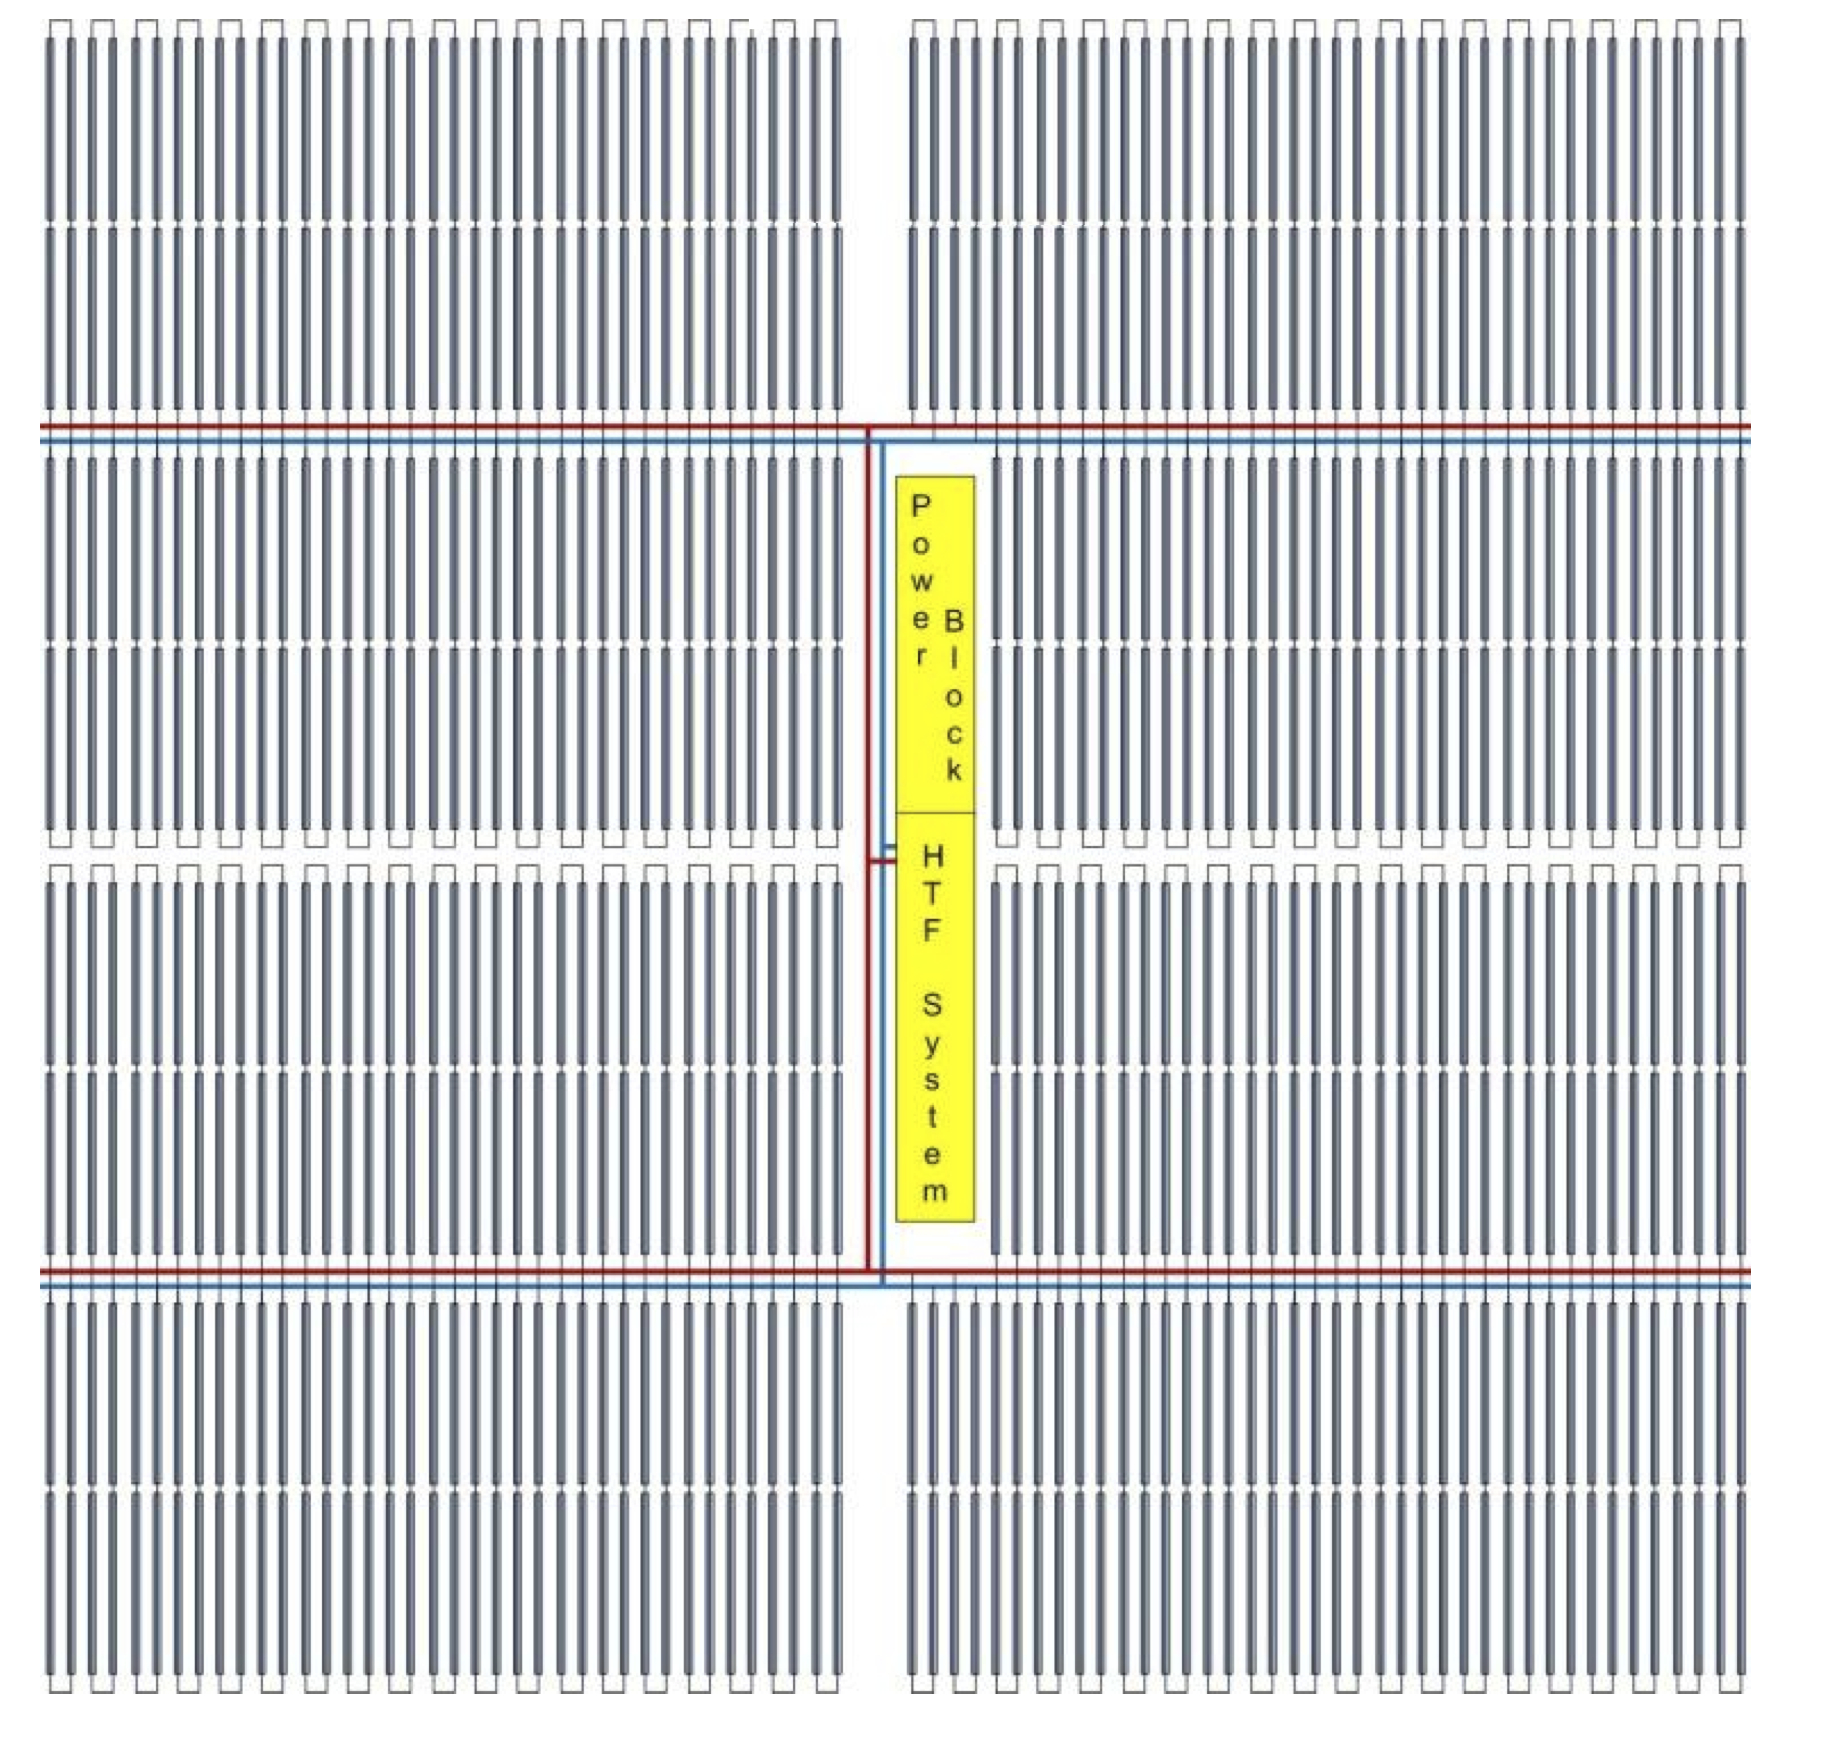
\includegraphics[width=0.7\linewidth]{FIG/PTC_field_EuroTrough}
\caption[Example of a EuroTrough collector field layout with 152 loops.]{Example of EuroTrough collector field layout with 152 loops \cite{VonReeken2014}.}\label{PTC_field_EuroTrough}
\end{figure}
Figure \ref{PTC_field_EuroTrough} shows one example plant layout for where  152 total loops are used, each loop with four SCA. The loop length depends on heat transfer fluid properties and rise in temperatures between inlet and outlet temperature ($\Delta T$). The flow rates through the receivers must be high enough to ensure appropriate heat removal from the absorber walls and low enough to keep pumping power for the fluid reasonably low.
\pagebreak
\subsubsection{Current stage of commercial scale PTC power plants}
On the commercial  scale the "Solana Generating Station" is currently one of the world largest PTC power plants. It was built from December 2010 to October 2013 southwest of Phoenix, Arizona. The solar-field aperture area of 2~200~000~m$^2$ concentrates in 808 loops with 4 SCA per loop drives two 140~MW$_{el}$ turbines. This plant uses synthetic oil as HTF and has a storage capacity of 6~h in molten salt (described in Chapter \ref{Subsection_storage_system}). The fed-in tariff of approx. 944~GWh/a is fixed for 30 years. The costs of the plant were approx. 2 USD billion. This power plant constitutes the current state of art in commercial scale PTC systems. \cite{NREL2015d}
\begin{figure}[!h] 
\centering
\includegraphics[width=1\linewidth]{FIG/PTC_Solana}
\caption[280-MW Solana PTC power plant near Phoenix, Arizona.]{280-MW Solana PTC power plant near Phoenix, Arizona \cite{AbengoaSolar2013a}.}\label{PTC_Solana}
\end{figure}
\pagebreak
\subsection{Central tower concentrating solar power} \label{subsection_CRS}
Central receiver systems (CRS) use a large number of reflectors (heliostats) to concentrate direct solar radiation to a focal point, in most cases on top of a tower. In order to reflect the incident sunlight to the focal point, the heliostats are tracked in two dimensions. The receiver is located at the focal point. The receiver absorbs the concentrated solar radiation and heats a HTF, such as a liquid or a gas. The generated heat drives a turbine to produce electricity by a generator. The basic principle of a solar CR power plant is shown schematically in Figure~\ref{power_tower}. Average concentration levels on the receiver are typically in the range 500-1~000 kW/m$^2$ \cite{Pitz-Paal.2013}. This concentration level is significantly higher than those achievable in linear focus systems such as PTC systems. The higher concentration level enables higher operational temperatures in the receiver, while maintaining good thermal efficiencies.
\begin{figure}[!h] 
\centering
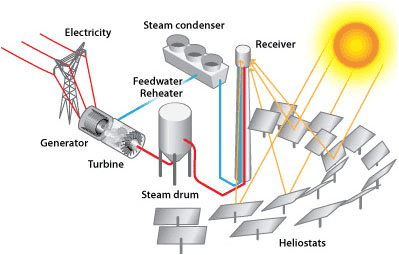
\includegraphics[width=0.6\linewidth]{FIG/power_tower}
\caption[Schematic CR power plant concept.]{Schematic CR power plant concept \cite{U.S.DOE2013}.}\label{power_tower}
\end{figure}


A variety of solar tower concepts exist or are under development. These concepts differ mainly in the type of heat transfer medium, which dominates the layout and selection of all other components except for the heliostat field. Liquid or gaseous HTFs are state-of-the-art in solar tower technology. Water/steam, molten salt, and air are typical fluids \cite{Pitz-Paal.2013}. A HTF in a central receiver absorbs the highly concentrated radiation reflected by the heliostats and converts it into thermal energy to be used for the subsequent generation of superheated steam for turbine operation. The different HTF mediums are described in  chapter \ref{subsection_HTF}. Not like the more or less uniform design of PTC systems is the optical design and optimization of CRS more complicated. A multitude of variables one must be consider such as the continuous variation in configuration and performance of each of the heliostats as they track the sun and interact with one another. 

The first documented concept of using ground-based segments (heliostats) to reflect direct-beam sunlight on a receiver comes from the Russian Victor Baum \cite{Baum1957}. But at this point no experimental device was built.

After several central receiver concepts and first 'commercial' used heliostats \cite{Trombe1957}, Alvin Hildebrandt published in 1972 the basic concept of nowadays CR systems as a hemispherical or cylindrical receiver atop a tall tower surrounded by a field of carefully positioned heliostats. The described power plant should have a tower height of 450~m with an heliostat field of 1.8~km diameter and produce 565~MW$_{th}$. There were no technical impediments expected with the tower or heliostat field. \cite{Hildebrandt1972}

Outgoing from more basic concepts and further research the Solar One, a 10~MW$_{el}$ CR ‘pilot plant’ was operated successfully from 1982 to 1988, in the desert near Barstow, California. This facility used a cylindrical receiver with water-steam as HTF at the focal point in 76~m height. The tower was surrounded by 1~818 heliostats, each with almost 40~m$^2$ area. After several problems in terms of storage and continuous turbine operation, the Solar One was upgraded to the Solar Two using molten salt as HTF and as direct storage concept. The Solar Two operated from 1996 to 1999 pumping molten nitrate salt at 290$\,^{\circ}\mathrm{C}$ from a cold storage tank through the receiver, where it was heated up to approximately 565$\,^{\circ}\mathrm{C}$ and afterwards to a storage tank, which had a storage capacity of 3~h. A simplified scheme of the Solar Two system is shown in Figure~\ref{towerdirecttwotank} on Page~\pageref{towerdirecttwotank}. \cite{Reilly2001}

The Planta Solar 10 (PS10) is the first solar central-receiver system producing grid-connected electricity under a purely commercial approach and started generating 11~MW$_{el}$ in 2007 near Seville, Spain. 624 heliostats with surface area of 120~m$^2$ each, concentrates direct irradiance to a cavity receiver using saturated steam as HTF on top of a 115~m high tower. The function of the PS10 is schematically shown in Figure~\ref{directsteamgeneration}.
\begin{figure}[!h] 
\centering
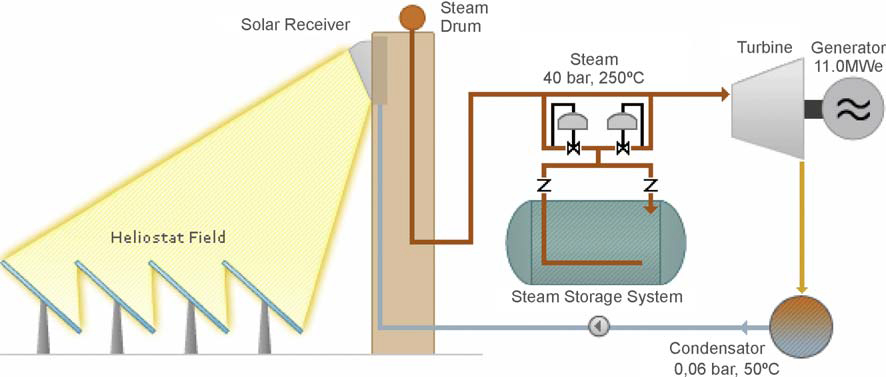
\includegraphics[width=0.7\linewidth]{FIG/directsteamgeneration}
\caption[Schematic diagram of the PS10 solar tower using water/steam as HTF.]{Schematic diagram of the PS10 solar tower using water/steam as HTF \cite{Medrano2010}.}\label{directsteamgeneration}
\end{figure}


The first commercial solar thermal power plant to supply uninterrupted power for a full 24~h is the 19.9~MW$_{el}$ Gemasolar power plant, which started operation also near Seville in 2011. 2~650 heliostats focusing on the tube receiver on top of a 140~m height tower. The molten salt, which is used as HTF and for storage, reaching temperatures of 565$\,^{\circ}\mathrm{C}$.

Current commercial planned large-scale CR power plants are based on the PS10 and the Gemasolar power plant. Their main components are the heliostats and their field design, the receiver, and the tower itself. These are described bellow. Chapter \ref{Subsection_storage_system} examined the storage possibilities.  \pagebreak
\subsubsection{Heliostats}
Current heliostat technology differs mainly in the area of the reflecting surface. Studies of the heliostats area reaches from 1.1~m$^2$ up to 320~m$^2$ \cite{Tyner2014,Blackmon2012}. One of the largest heliostats in commercial application will have a total area of 140 m$^2$ \cite{Abengoa2014} and are built of several smaller facets, mounted on a back structure. Classical heliostat design is dominated by mirrors brought into position by steel structures and drives that guarantee high accuracies under wind loads and thermal stress situations. To the structures that hold the mirrors include struts, beams, the pylon, and the foundation. The linear actuators enable moving of the heliostat in two dimensions. There exists a zenith and an azimuth actuator together with their step motors. The orientation of the rotation axes may also differ between heliostat types. Several different types of heliostat mirrors exist. They can be differentiated according to size, shape, basic design concept, or even according to there tracking system. Each heliostat type has its own characteristics in terms of wind-performance and tracking during windy conditions, costs, and complexity of control. A field made up of more small heliostats will require a more complex control system than a field of fewer heliostats. Therby, large heliostats are mostly more cost-efficient than small ones (see Figure \ref{Heliostats}). Improvements in controllability may cause this to change, however, and several companies are attempting the strategy of many small heliostats as opposed to fewer large heliostats.
\begin{figure}[!h] 
\centering
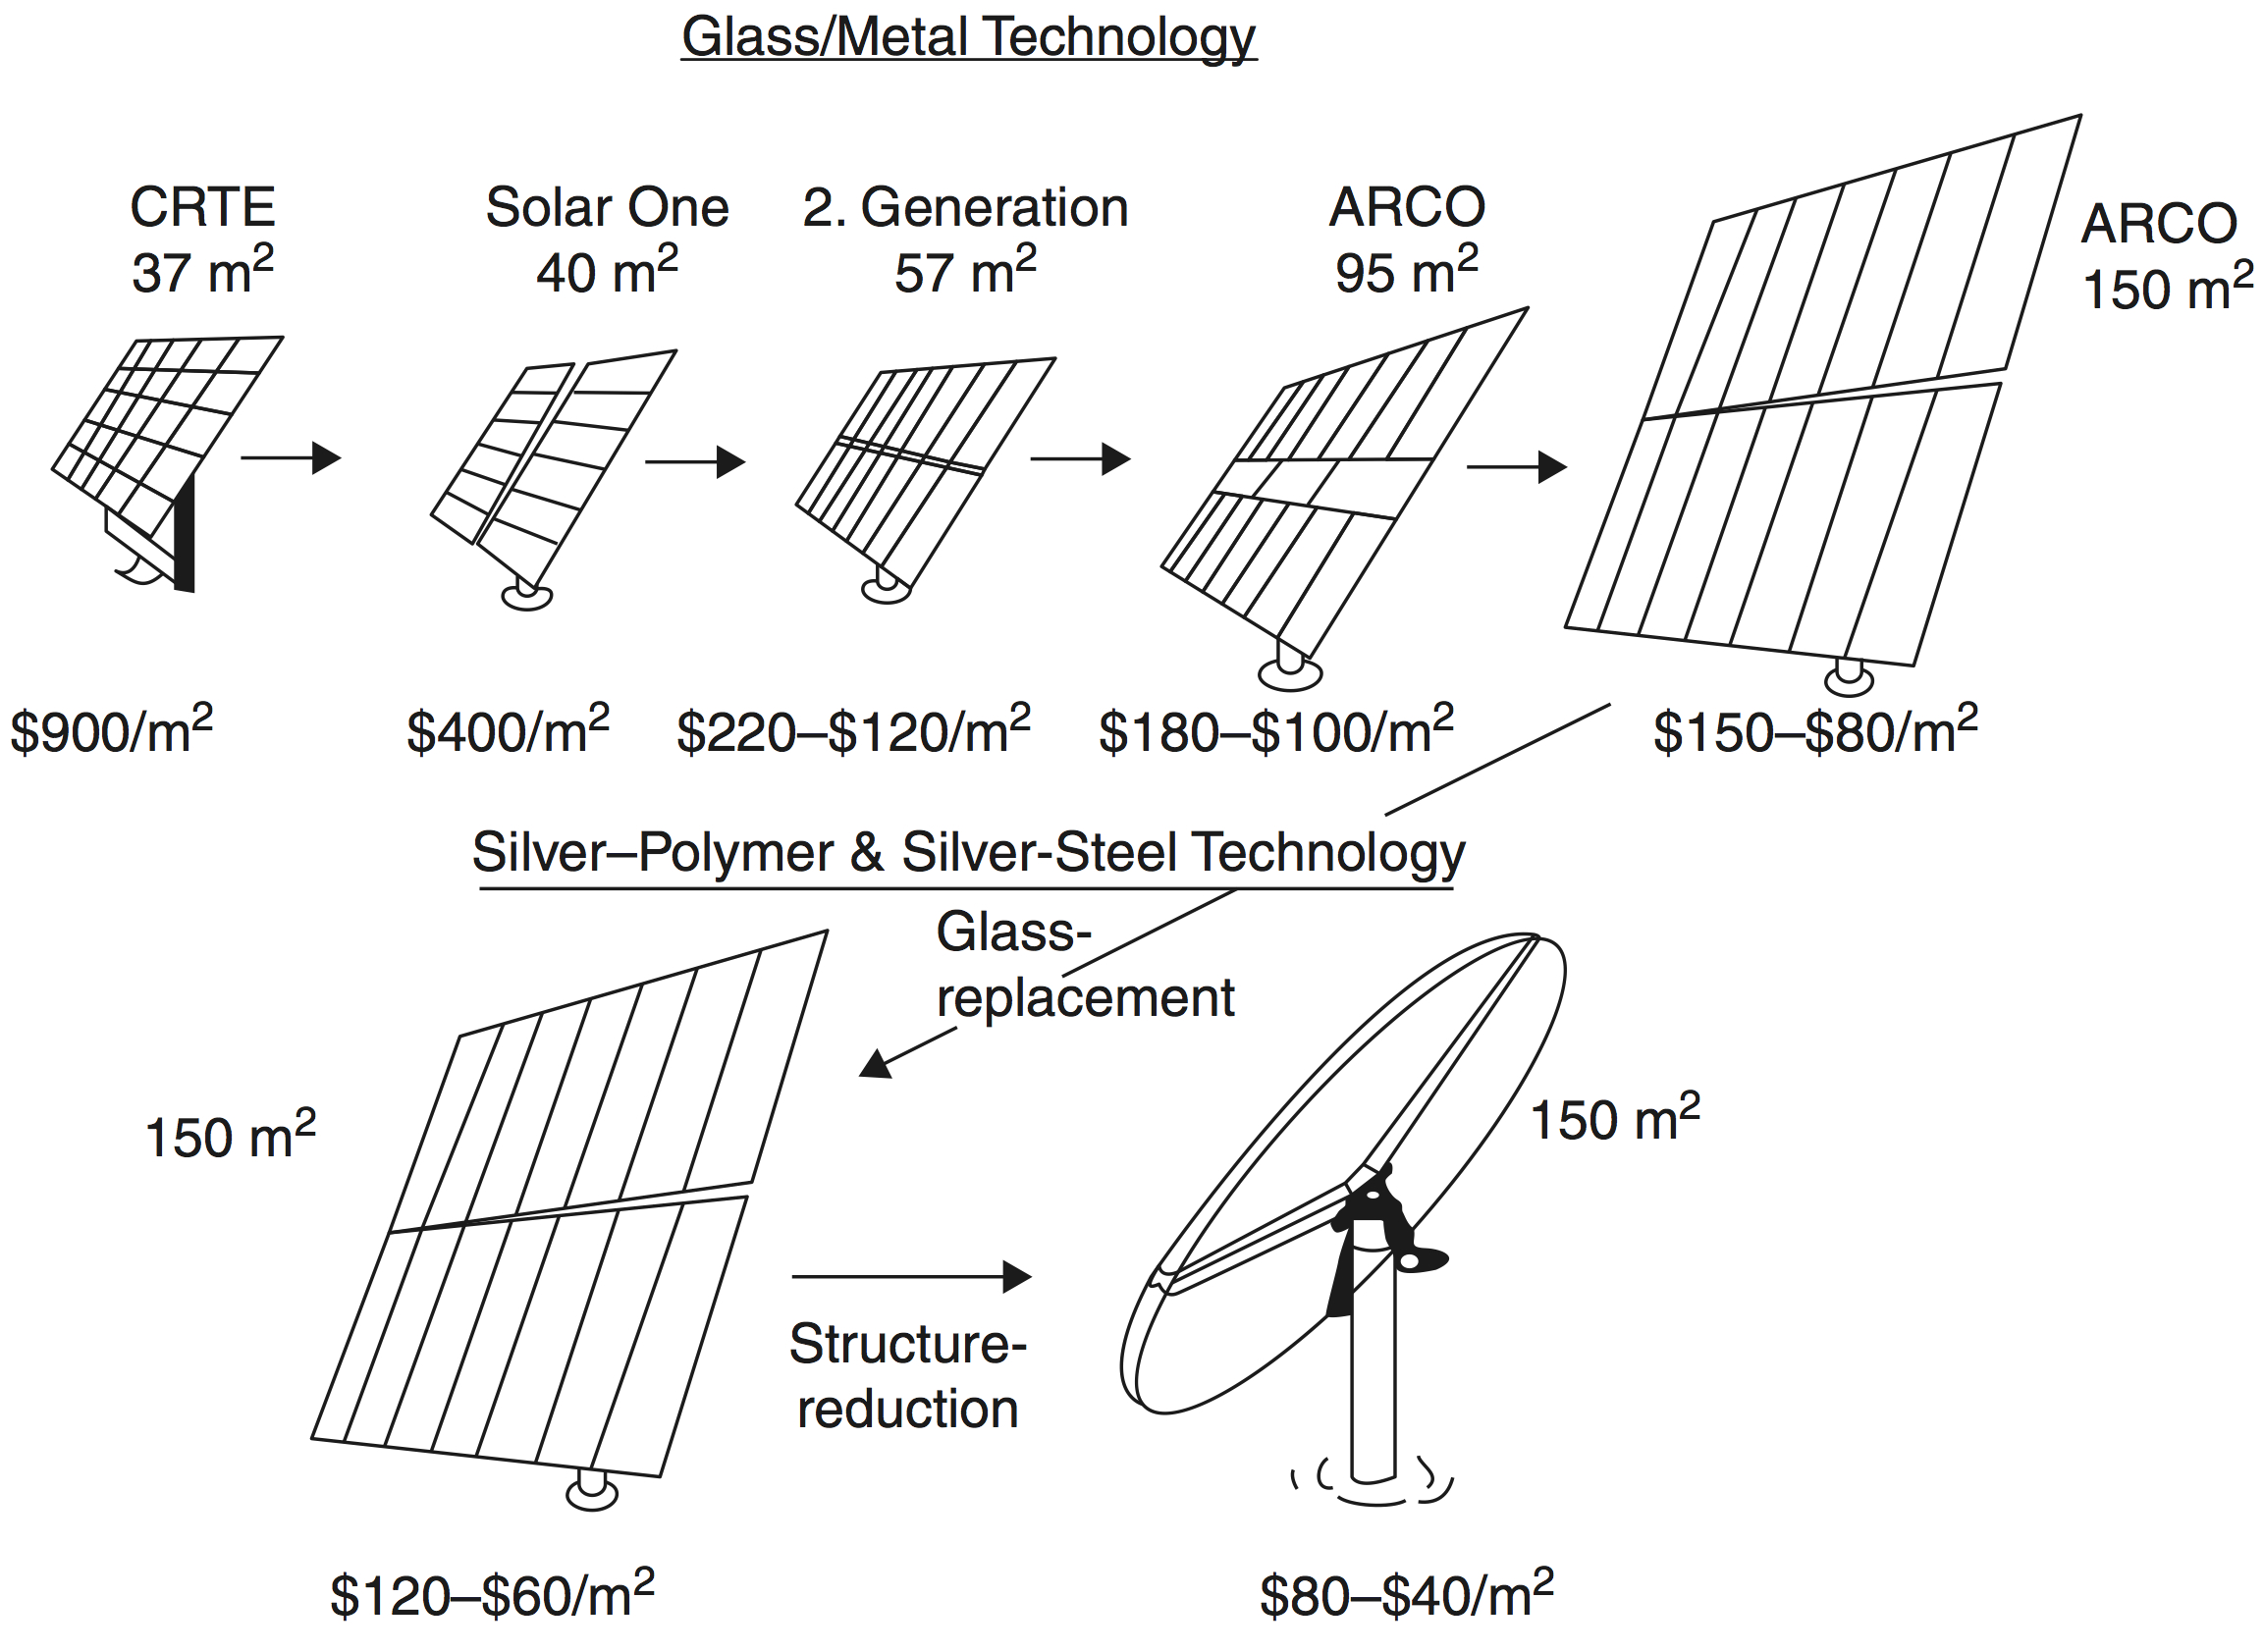
\includegraphics[width=0.9\linewidth]{FIG/Heliostats}
\caption[Heliostats used in solar power plants and their costs.]{Heliostats used in solar power plants and their costs \cite{Kolb2007}.}\label{Heliostats}
\end{figure}
\subsubsection{Heliostat field design}
The heliostat field layout is a complex topic. Decisions regarding the best position for locating heliostats relative to the receiver and how high to place the receiver above the field constitute a multifaceted problem, in which costs and heliostat loss mechanisms are among the variables, and which is solved by an iterative process. Therefore the location and the receiver type is decisive. In the northern hemisphere, the position of the sun is to the south of the plant and the field must be placed to the north of the tower. In the southern hemisphere the opposite is true. The general terminology for this position would be the "polar side" of the tower, which can be applied to towers in both the northern and southern hemispheres. The opposite side of the tower is the
"equatorial side" \cite{Alexopoulos2013}. The basically distinguishable field design types are shown in Figure \ref{Fielddesign} and can either surround the tower (Surround-field) for larger systems or be spread out on the shadow side of the tower (Polar-field) in the case of smaller systems.
\begin{figure}[!htbp]
        \centering
        \begin{subfigure}[b]{0.5\textwidth}
                \centering
                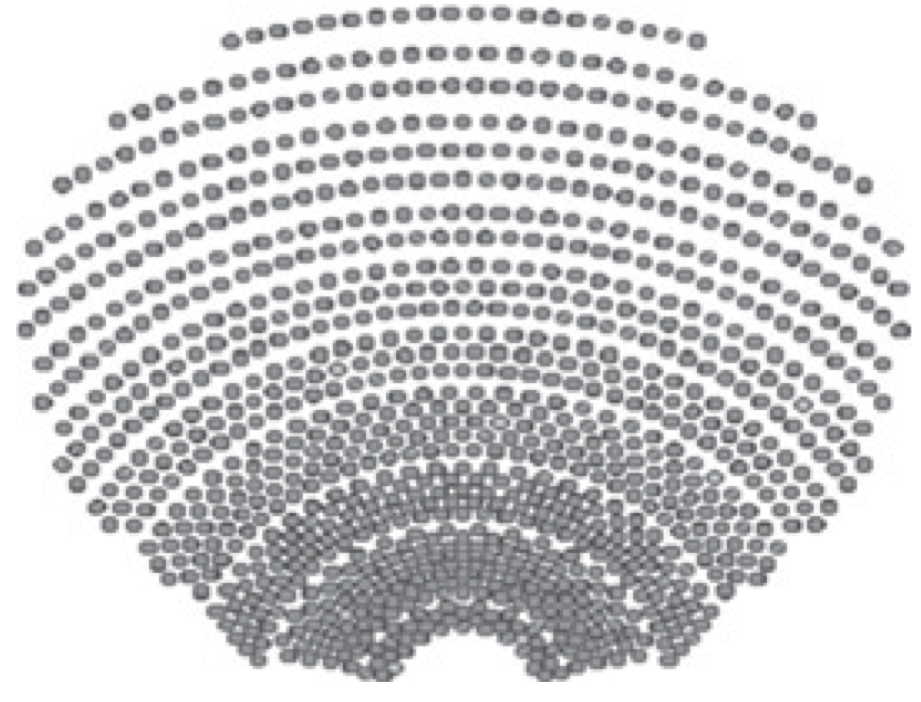
\includegraphics[width=0.9\textwidth]{FIG/north_field_layout}
                \caption{Polar-field layout.}\label{north_field_layout}
        \end{subfigure}%
        ~
        \begin{subfigure}[b]{0.5\textwidth}
                \centering
                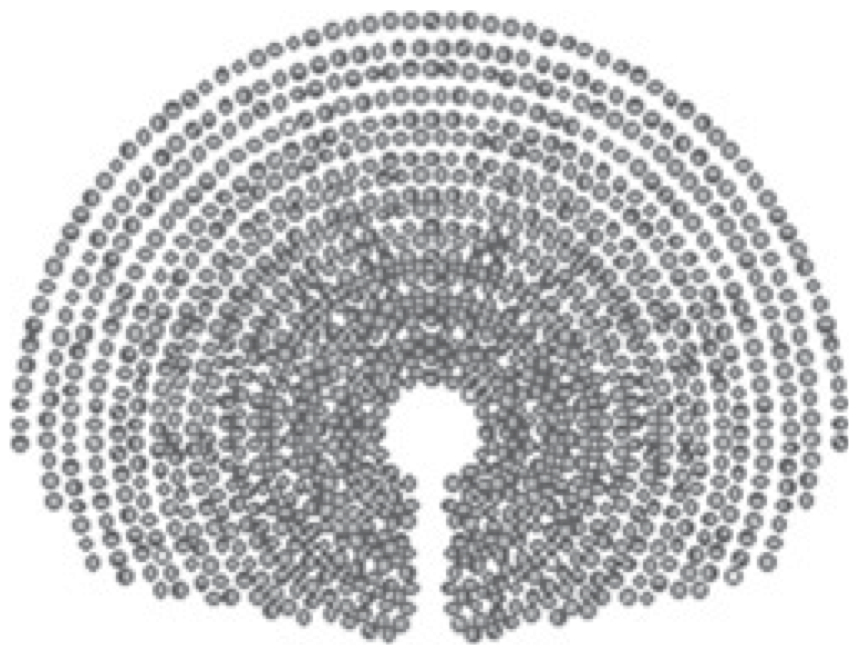
\includegraphics[width=0.9\textwidth]{FIG/sourround_field_layout}
                \caption{Surround-field layout.}\label{sourround_field_layout}
        \end{subfigure}
        \caption[Basically distinguishable field design types.]{Basically distinguishable field design types \cite{Kulichenko2012}.}\label{Fielddesign}
\end{figure}
With a field on only one side of the tower, a cavity receiver is usually used. Close to the equator, where the sun passes directly overhead, a surrounding-field can be used in combination with an open receiver (Tube receiver, see below). Another possibility is the use of two ore three fields – one on either side of the tower, in combination with a cavity receiver for each side (see Figure \ref{KhiSolarOneReceiver}). With higher power levels, surround field layouts are usually more economical. The higher the site latitude of a plant (i.e., the further away from the equator), the more the heliostat field tends to be shifted polewards. When laying out a heliostat field there are several types of losses that must be considered. These are not only the optical losses, so called, the cosine losses and losses due to shadowing, blocking, spillage (reflected radiation miss the receiver surface), and atmospheric attenuation, but also technical considerations, that is, the mirror reflectivity, mirror surface defects, tracking accuracy, wind load, and tower oscillations (due to wind load) as well as the heliostat fault rate. The aim in the designing of a heliostat field is to reliably produce the power required by the power block whilst keeping land usage and total costs to a minimum. \cite{Vant-Hull2012} \pagebreak
\subsubsection{Tower and receiver}
The function of the tower is to positioning the receiver in the required height above the heliostat field. So the choice of tower constructions depends primarily on the required height of the tower. But the height of the tower is limited by its cost. Towers are mainly constructed of steel or reinforced concrete. 



The function of a receiver is to absorb the concentrated solar irradiation energy impinging from the heliostat field and transfer it to the working fluid. Requirements to a solar receiver include high thermal conductivity, dark color of the body for high absorptivity, and temperature resistance. According to Prof. Dr. Hoffschmidt \cite{Hoffschmidt2014} from the German aerospace center (DLR) there are actually two main receiver types state of art for CR power plants, which uses molten salt and water for direct steam generation: external (tube) receiver and cavity receiver. 
\begin{figure}[!htbp]
        \centering
        \begin{subfigure}[b]{0.5\textwidth}
                \centering
                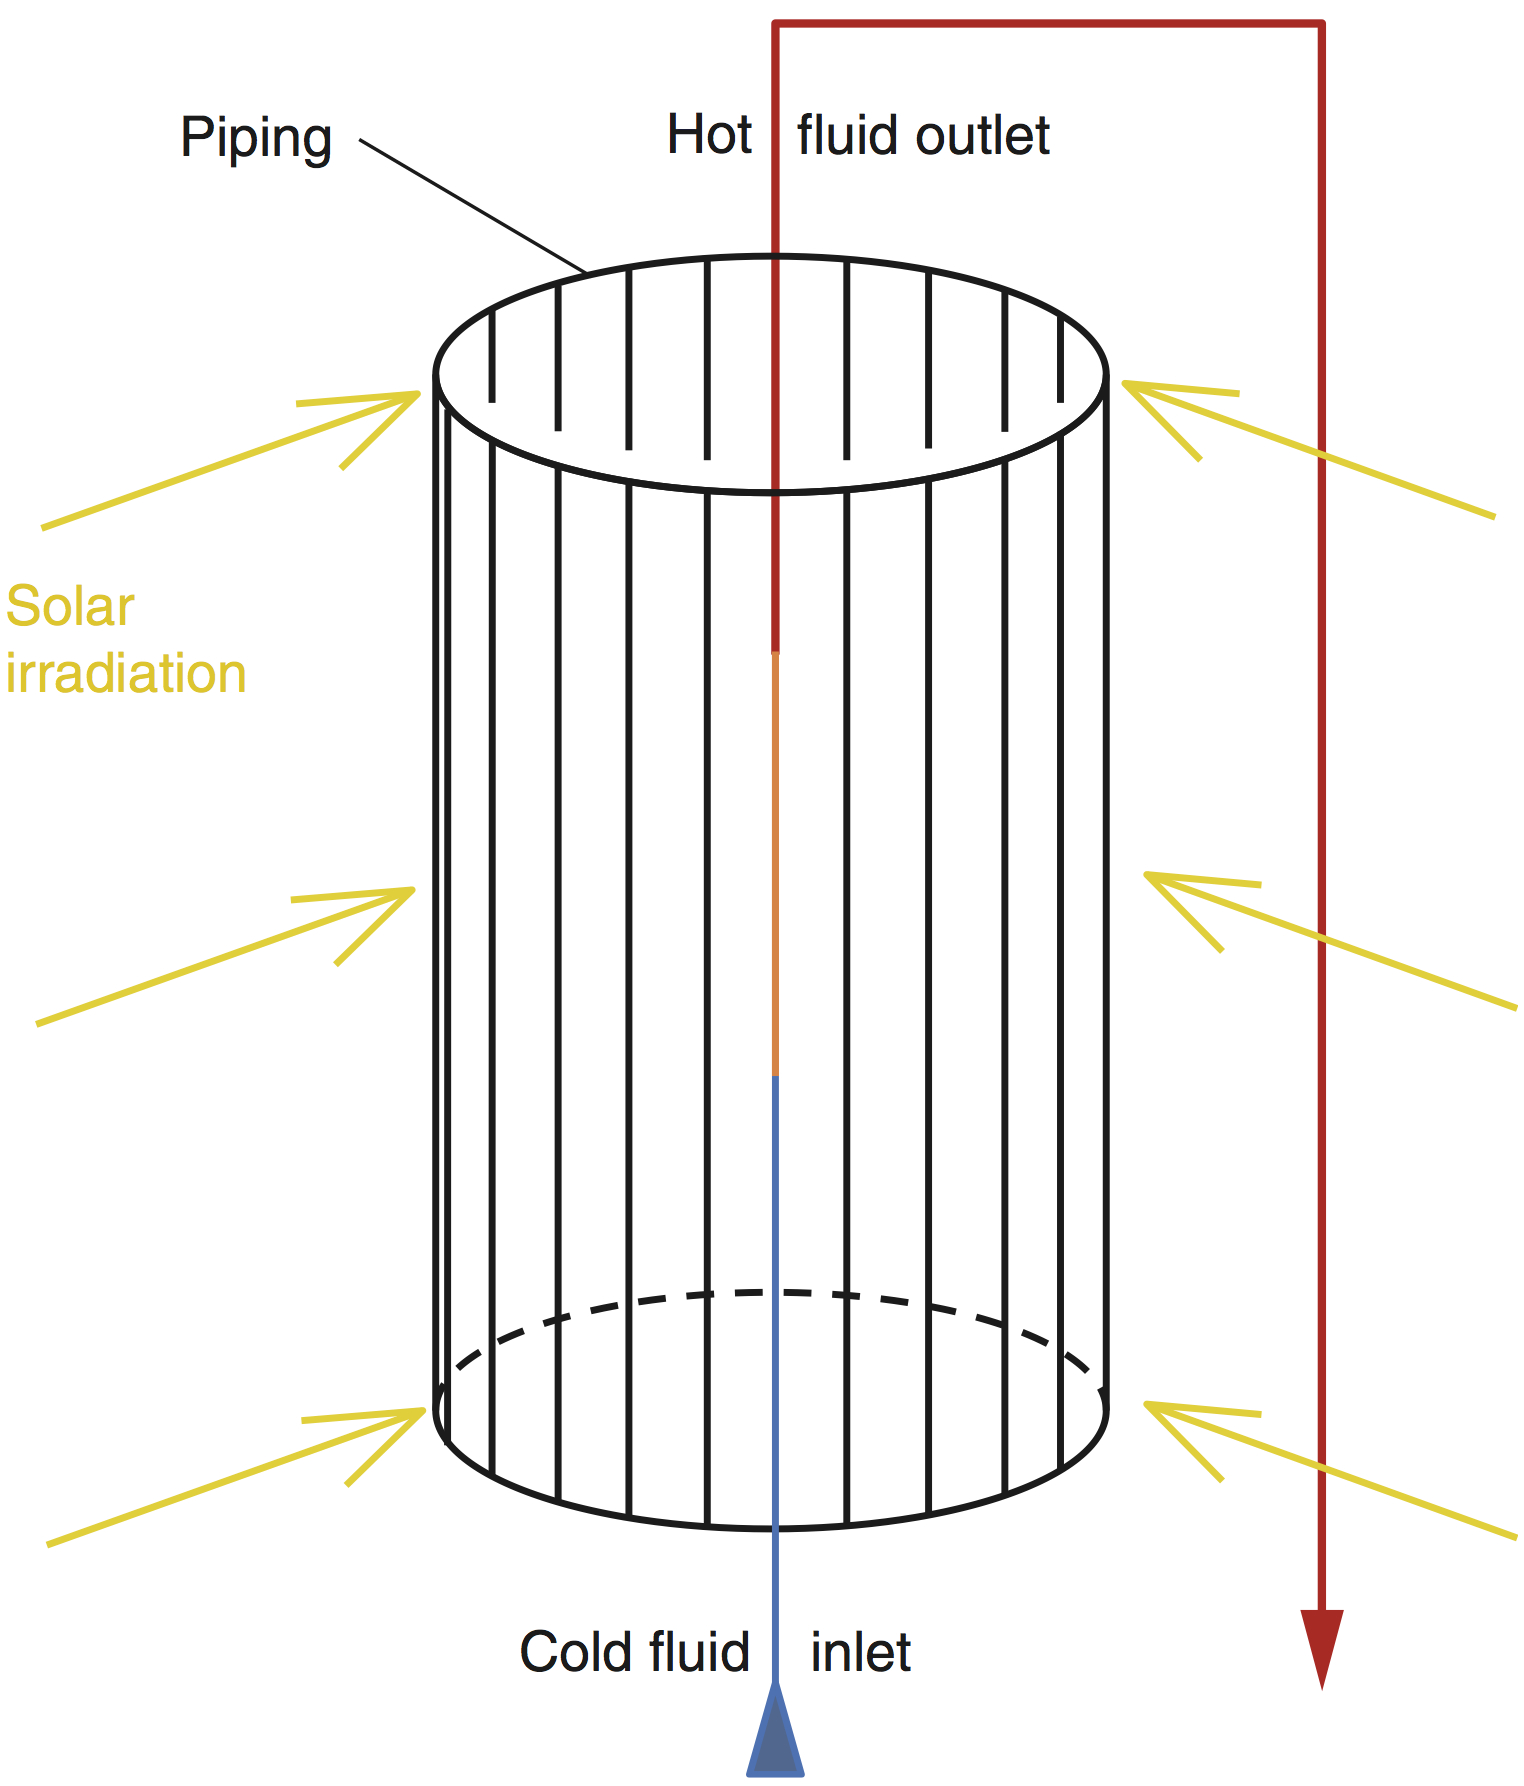
\includegraphics[width=0.9\textwidth]{FIG/TubeReceiver}
                \caption{External tube receiver concept \cite{Alexopoulos2013}.}\label{TubeReceiver}
        \end{subfigure}%
        ~
        \begin{subfigure}[b]{0.5\textwidth}
                \centering
                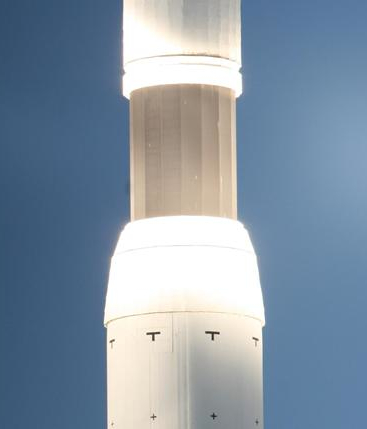
\includegraphics[width=0.9\textwidth]{FIG/Gemasolar_tower_heatshield}
                \caption{External tube receiver implemented in Gemasolar power plant \cite{Microtherm2012}.}\label{Gemasolar_tower_heatshield}
        \end{subfigure}
        \caption[External tube receiver concept and example of application.]{External tube receiver concept and example of application.}\label{TubeReceiverConceptGemasolar}
\end{figure}


An external receiver consists a large number of vertically arranged pipes or flat plates through which the HTF is pumped in upward direction. There are variations of shapes for the external receiver, mostly cylindrical or square-shaped. The tubes in the receiver can be crosswise arranged with different zones for pre-heating, evaporation and superheating (in case of super heated steam). Typical solar heat fluxes in this type of receiver are up to 1 MW/m$^2$ \cite{Pitz-Paal.2013}. An basic concept for an external receiver is shown in Figure \ref{TubeReceiver} with a cylindrical shape. An example for such a external tube receiver is the receiver of the Gemasolar power plant, that used molten salt as HTF. The receiver consists of a great number of HTF pipes. The external receiver pipes are fixed vertically whereby the salt smelt is pumped in upward direction. The receiver outlet temperature of the molten salt is approximately 565$\,^{\circ}\mathrm{C}$. The tube receiver of the Gemasolar power plant is shown in Figure \ref{Gemasolar_tower_heatshield}. An other example  is the Ivanpah Solar Electric Generating System (ISEGS) in California’s Mojave Desert where they produce direct steam at 550$\,^{\circ}\mathrm{C}$ using an external tube receiver which is square-shaped. A disadvantage for using the pipe receiver is the high reflection loss which is higher than for other receiver types. One way to reach reduction of thermal losses is an cavity arrangement and a face down arrangement. \cite{Hoffschmidt2014}
\begin{figure}[!htbp]
        \centering
        \begin{subfigure}[b]{0.5\textwidth}
                \centering
                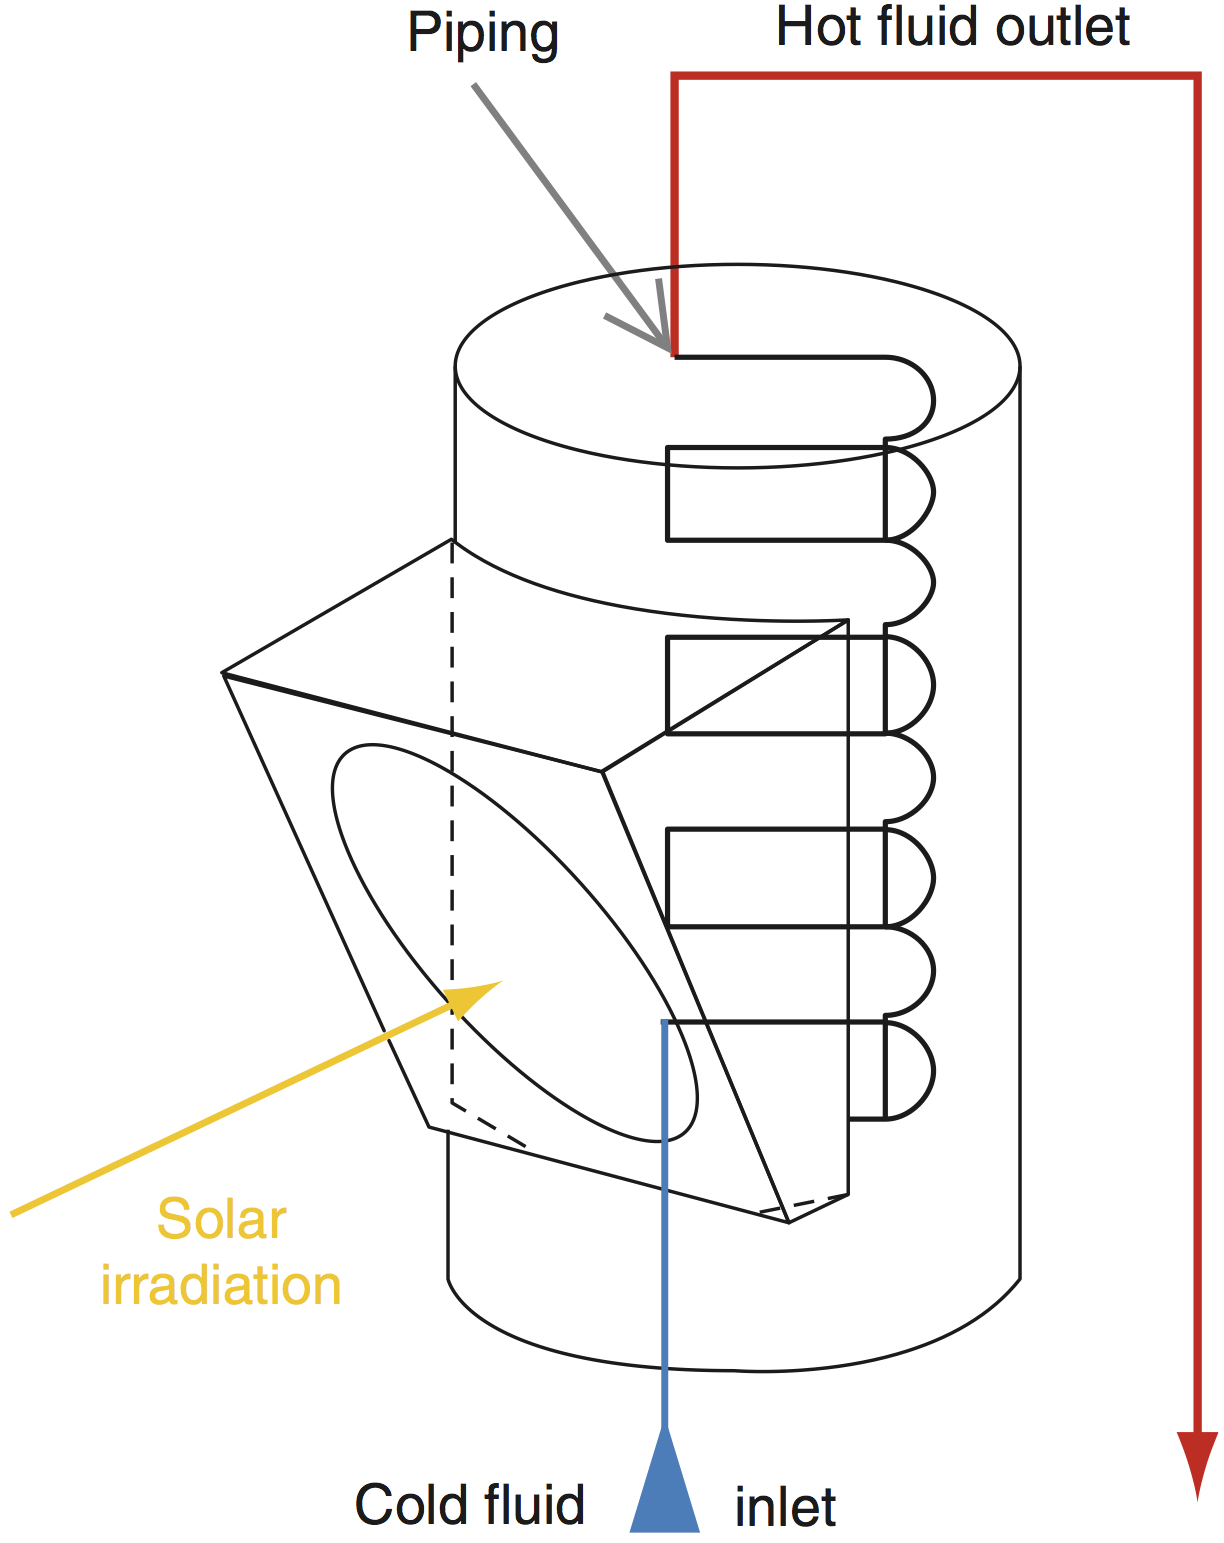
\includegraphics[width=0.9\textwidth]{FIG/CavityReceiver}
                \caption{Basic cavity receiver concept \cite{Alexopoulos2013}.}\label{CavityReceiver}
        \end{subfigure}%
        ~
        \begin{subfigure}[b]{0.5\textwidth}
                \centering
                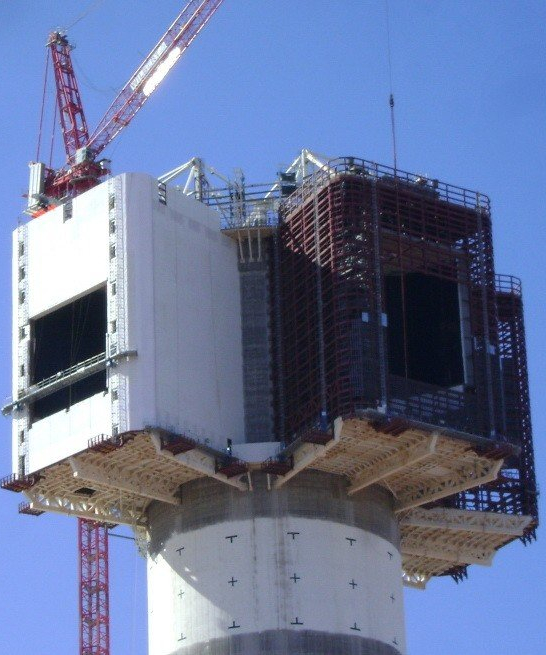
\includegraphics[width=0.9\textwidth]{FIG/KhiSolarOneReceiver}
                \caption{Three under construction situated cavity receiver mounted at the  Khi Solar One Tower \cite{CMI_Energy2015}.}\label{KhiSolarOneReceiver}
        \end{subfigure}
        \caption[Cacity receiver concept and example of application.]{Cavity receiver concept and example of application.}\label{CavityReceiverConceptKhiSolar}
\end{figure}


A cavity receiver consists of a cavity with a small opening where the receiver is located. The concentrated solar irradiation is directed into the small opening where it impinges on tubes carrying the working fluid. The idea of the cavity receiver is the reduction of thermal and optical losses. From the radiation entering the inlet aperture, only small amounts are reflected back into the atmosphere through the inlet aperture. Figure \ref{CavityReceiver} shows the basic concept of an cavity receiver. The cavity receiver concept is implemented in the PS10 solar tower plant in Spain. The direct irradiated absorber tubes is basically a forced circulation radiant boiler with low ratio of steam at the panels output, which produce saturated steam at 250$\,^{\circ}\mathrm{C}$ and 40~bar. A schematic diagram of the PS10 is shown in Figure \ref{directsteamgeneration}. SA first solar power tower will also use a cavity receiver technology. Figure \ref{KhiSolarOneReceiver} shows the three under construction situated cavity receiver of the Khi Solar One. Two steam generator (east and west orientated) and one super heater (south orientated) using the cavity receiver concept are external mounted on the tower \cite{Prof.Dinter2015}.
\subsubsection{Current stage of commercial scale CR power plants}
As shown above there is a variety of CR concepts also for commercial scale. But there are three outstanding CR projects worth mentioning for large-scale commercial application. The Khi Solar One, the Ivanpah Solar Electric Generating System (ISEGS) and the Atacama-1.



Fore SA obviously the Khi Solar One, which will be the first commercial scale CR power plant in the country. This 50.0~MW$_{el}$ power tower is under construction and will be operated by Abengoa Solar. The Polar-field consists out of 4~120 heliostats with a reflection surface of 140.0~m$^2$ each concentrate direct solar irradiance on three cavity receiver. \cite{NREL2014,Prof.Dinter2015}



The Ivanpah Solar Electric Generating System (ISEGS) is currently the largest CSP plant operating by BrightSource. The three-unit power system with in total 377.0~MW was started operation 2014 in Ivanpah Dry Lake, California. The three external square-shaped receiver on each tower are focused by 173~500 heliostats with a aperture area of 15.0~m$^2$ each. The costs for the power plant which consists out of three CRS are approx. 2~200~USD million. But instead of an storage system BrightSource using a natural gas fired backup for the ISEGS. \cite{BrightSourceEnergy2014,NREL2014a}



One of the highly promising CR projects for large-scale commercial application is Abengoa Solars Atacama-1. The eponymous Atacama desert in Chile, where the plant is under construction, has the highest levels of solar radiation worldwide. The scheduled operation start of the plant is in 2018. 10~600~heliostats each 140~m$^2$ in aperture area will concentrate on a external cylindrical shaped receiver with 32~m in height and 19~m in diameter. The receiver will be positioned in a 243~m-tower to heat molten salt to drive a 110~MW$_{el}$ steam turbine and 17.5~h direct thermal storage. This will generate electricity 24~h per day, similar to the Gemasolar power plant, but more than five times that powerful. This project constitutes the current state of art in commercial scale CRS. \cite{NREL2015b,AbengoaSolar2015a,AbengoaSolar2015}
\pagebreak
\subsection{Heat transfer fluid} \label{subsection_HTF}
In each CSP family, various options exist for the heat transfer fluid, the storage technology, and the thermodynamic cycle. The heat transfer fluid (HTF) removes heat from the receiver and transfer it either to the storage system or to the final use. The correct choice of the fluid is determinant in order to reduce costs and increase the efficiency of the plant. The most important HTFs are:
\begin{itemize}
\item \textbf{Synthetic oils} They are used predominant in PTCs thanks to their low pumping losses, their adequate conductivity and the fact that they do not need very high pressures, around 16 bar. However, they face a temperature limit of 393$\,^{\circ}\mathrm{C}$, which limits the efficiency of the plant. In addition, they are toxic and flammable.
\item \textbf{Direct steam generation} If saturated or superheated steam is generated directly at the receiver two main advantages are found: first, no heat exchanger is required in order to generate steam from the HTF and second, the exergy loss that takes place at such heat exchanger is avoided. However, some issues are also found: high pressures are required, which makes it not suitable for PTC's due to leakages at the movable elements, different thermal regimes are found in the steam generation, which complicates transients and superheating, and no efficient method has been found for energy storage. This last point is a main issue, especially when the importance of dispatchability is considered.
\item \textbf{Molten salts} Molten salts are playing a great role in CSP for energy storage. The most commercial molten salts have a working temperature range from 290$\,^{\circ}\mathrm{C}$ to 565$\,^{\circ}\mathrm{C}$, and thus higher efficiencies are obtained at the power block (cf. Table \ref{TableSensbleHeatStorageMaterial}). However, they have the issue of solidifying at relative high temperatures. As a result, if the receiver cannot be evacuated when there is no impinging sun, which is the working mechanisms in central towers with molten salts, the fluid must be recirculated from the hot tank to the cold tank, increasing thermal energy losses. Evacuation of linear receivers seems more difficult than in central towers due to the fact that tubes are horizontal.
\item \textbf{Pressurized gasses} Gasses do not have any limit in temperature, neither by the upper nor by the bottom part. In addition, they are cheap, especially if the air is used as it is found in the atmosphere. However, pumping losses are much higher than in liquid HTFs due to the density difference. In order to overcome this issue, pressure must be increased, pumping power losses being inversely proportional to the squared power of the pressure. At current time no commercial power station uses pressurized gases, although they have been used in central tower (Solgate) and CCP research prototypes. Leakages of the gas found in the movable elements of PTCs due to the high pressures suggest the need of fixed receivers in order to use pressurized gasses.
\end{itemize}
\subsection{Storage systems for CSP}\label{Subsection_storage_system}
The storage systems plays the decisive role that makes solar thermal power stand out from other renewable energy technologies. By the integration of heat storage capacity, STP plants are actually the only operational renewable energy option on the market offering dispatchable electricity power generation in multi-MW range. With the thermal energy storage (TES) system a CSP power plant offers the advantage of an integrated solution, which does not impose additional requirement on the electrical grid. Figure~\ref{integratedstoragescheme} shows the general scheme to store thermal energy into a CSP plant. The storage unit is connected both to the solar receiver and the power block. During charging the heat (high enthalpy mass flow) from the solar receiver is transferred to the thermal cycle, while the storage unit is charged by excess thermal heat. During the discharge process, the working fluid of the power block is heated by the energy from the  storage systems. Alone or in combination with some fossil fuel backup, the storage system keeps the plant running under full-load conditions. The energy from the storage might be also used to preheat the collector system during the ramp up time of the power plant.
\begin{figure}[h] 
\centering
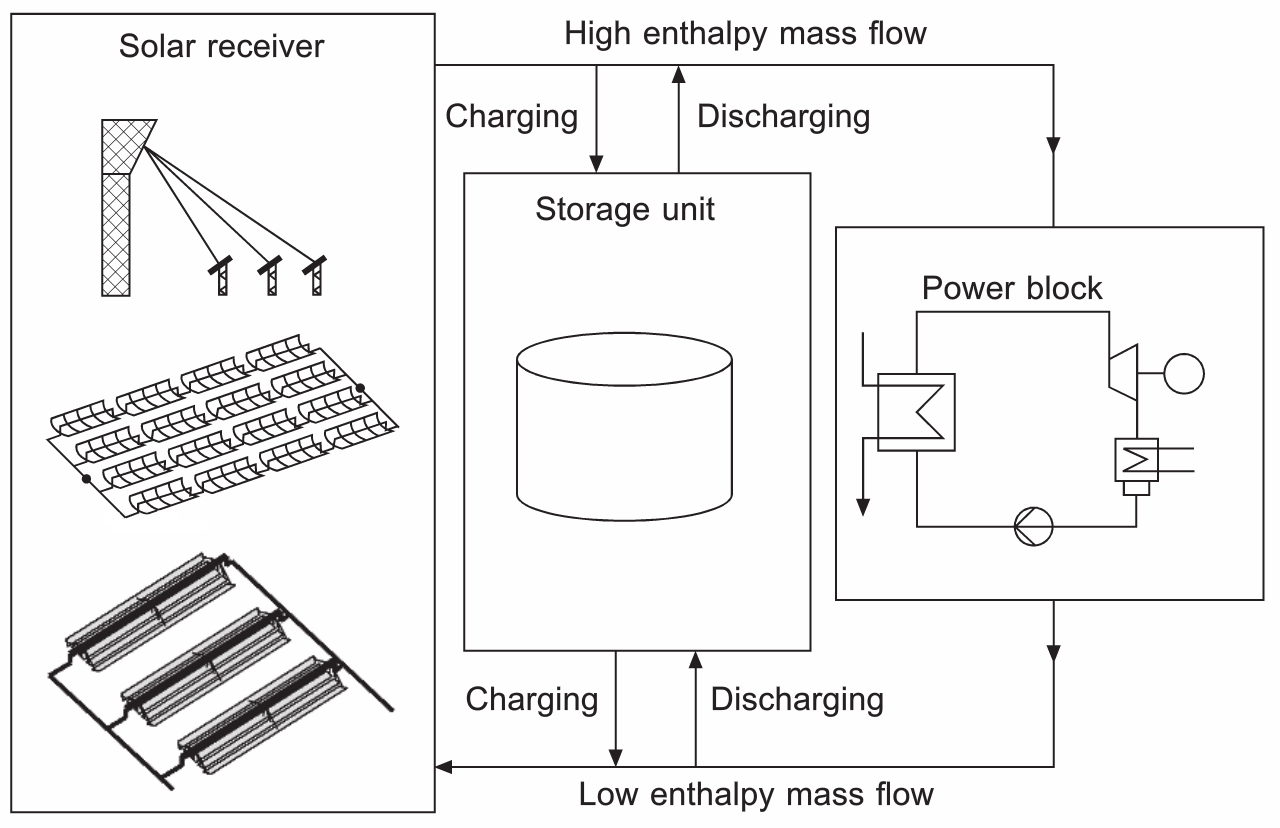
\includegraphics[width=0.70\linewidth]{FIG/integratedstoragescheme}
\caption[Scheme for CSP plant with integrated storage unit.]{Scheme for CSP plant with integrated storage unit \cite{Steinmann2015}.}\label{integratedstoragescheme}
\end{figure}
From a technical point of view, the storage must have high energy density, good heat transfer between the heat transfer fluid (HTF) and the storage medium, mechanically and chemically stable storage media, compatibility between the heat exchanger, heat transfer fluid and storage medium, complete reversibility, and minimum thermal losses. Actually, there are just four commercial used TES in CSP plants integrated (see below). But in generally a TES system, can store heat in the form of sensible, latent, or thermochemical energy. Latent and thermochemical based TES systems are still in the phase of research and development \cite{Steinmann2015}.
\begin{figure}[t]  
\centering
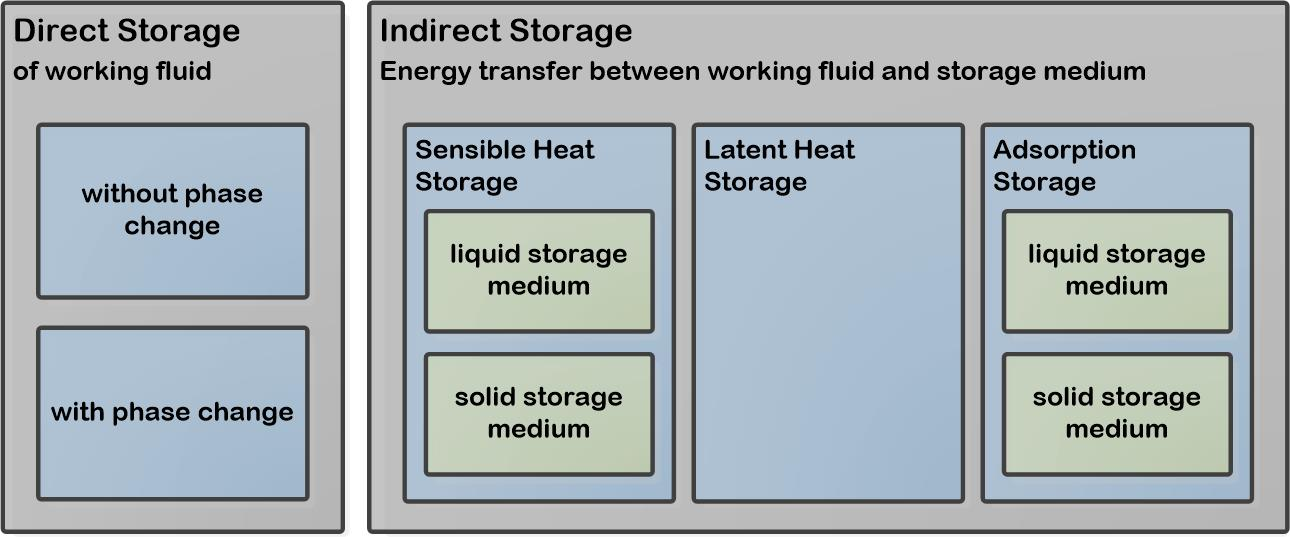
\includegraphics[width=0.75\linewidth]{FIG/Basicstorageconcepts}
\caption[Basic storage concepts for CSP systems.]{Basic storage concepts for CSP systems.}\label{Basicstorageconcepts}
\end{figure}


In Figure~\ref{Basicstorageconcepts} is on one site the more basic concepts for a direct storage shown, which use the same working fluid for the storage system and the solar receiver and on the other site indirect systems transferring energy to a separate storage medium. The various storage concepts show different states of maturity. These commercial integrated storage systems and their application range will described in the following \cite{Steinmann2015}:
\begin{itemize}
\item Direct storage of heat transfer oil (Direct Storage of Liquid Working Fluid)
\item Indirect molten salt storage units (Indirect Storage in Liquid Media)
\item Steam accumulators (Direct Storage with Phase Change)
\item Direct molten salt storage units (Direct Storage of Liquid Working Fluid)
\end{itemize}
According to the "Technology Roadmap - Energy storage" of the International Energy Agency from 2014, alternative storage concept like heat storage with phase changing materials (PCM), thermochemical energy storage, and waste heat utilisation methods offer many potential opportunities. However, these technologies will need to overcome containment vessel design and material stability challenges at very high temperatures before they can achieve widespread deployment and will not further described or disused here. \cite{IEA2014e}

Likewise alternative concepts in liquid storage media such as dual media concepts (thermocline) and floating barrier concepts are still in the phase of research and development and will not be further described.\cite{Steinmann2015} 



In the following sensible liquid media will be described. Therefor the physical principles of heat storage systems are necessary. The amount of heat, $Q$ (in J), which can be stored in liquid sensible systems and the density, $E$ (J/m$^3$), related with this process can be calculated using the following equations:
\begin{align}
Q=m*C_p*(T_{out}-T_{in})=m*C_p*\Delta T \label{GL_heat}
\end{align}
\begin{align}
E=\rho*C_p*(T_{out}-T_{in})=\rho*C_p*\Delta T \label{GL_density}
\end{align}
where $T_{in}$ and $T_{out}$ are inlet and outlet storage system temperatures, respectively [K], $m$ is mass of storage liquid media [kg], $\rho$ is density [kg/m$^3$], and $C_p$ is specific heat capacity [J/(kg*K)]. Analyzing equation \ref{GL_heat} and \ref{GL_density}, it can be concluded that an optimum liquid sensible storage material must present high heat capacity, $C_p$, and a wide range of thermal stability, $\Delta T$. Different fluids have been studied as HTF and liquid sensible storage media \cite{Gil2010} and are shown in Table \ref{TableSensbleHeatStorageMaterial}. \cite{Ushak2015}
\begin{table}[h]
\centering
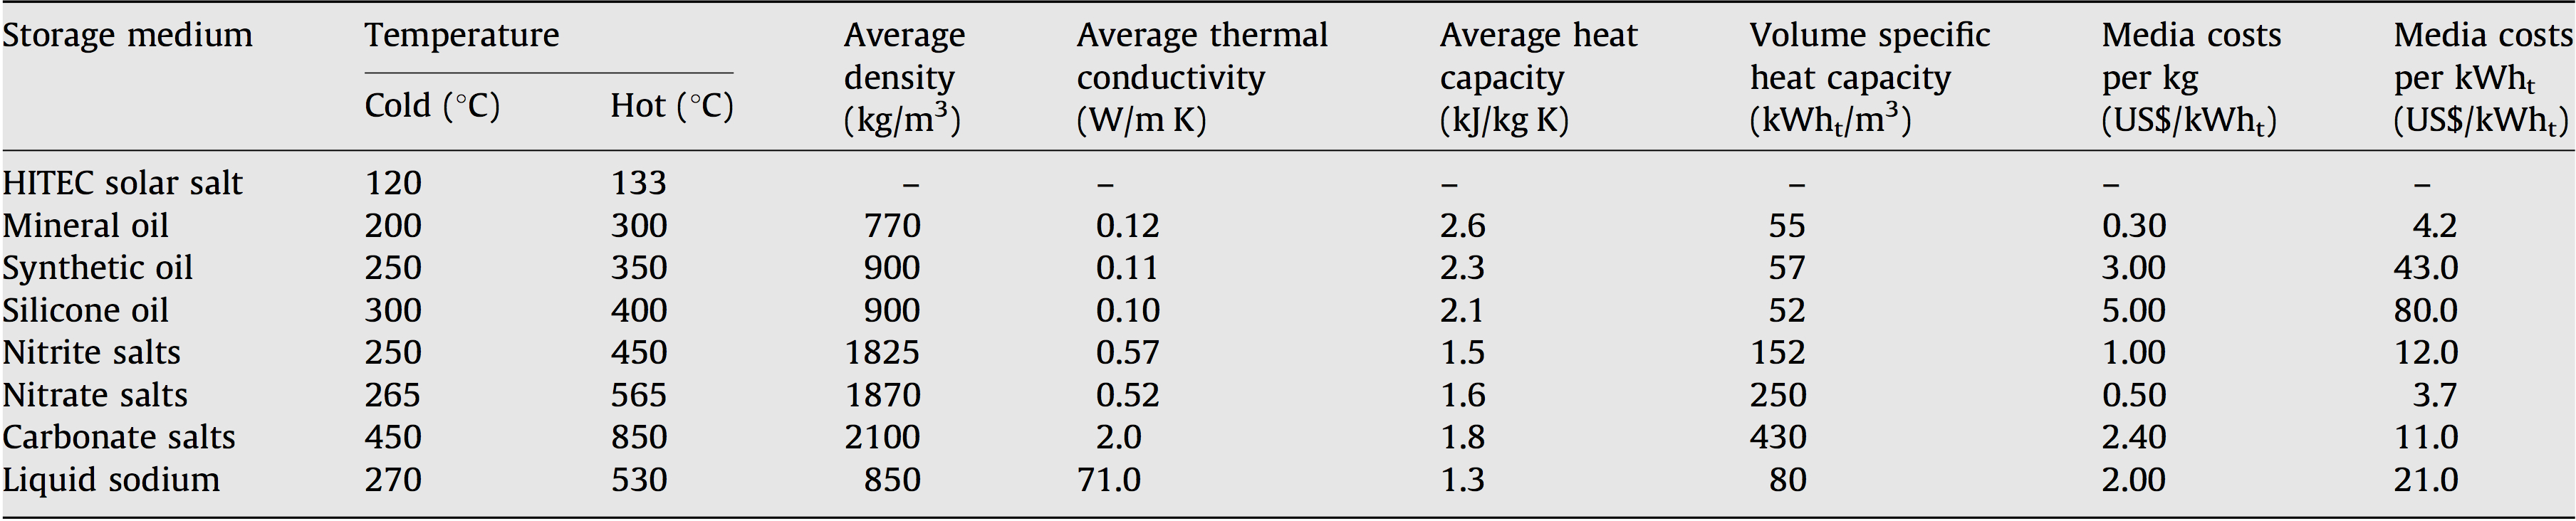
\includegraphics[width=1\textwidth]{FIG/TableSensbleHeatStorageMaterial}
\caption[Main characteristics of sensible heat storage liquid materials.]{Main characteristics of sensible heat storage liquid materials \cite{Gil2010}.}\label{TableSensbleHeatStorageMaterial}
\end{table}
\subsubsection{Direct storage of heat transfer oil}
The simplest concept to implement a TES into a CSP plant is the direct storage of the working fluid which is circulated through the solar absorbers. The first commercial used parabolic trough power plant SEGS-1, built 1984 in California, uses a mineral oil as heat transfer medium in the absorbers, which heats up from 240$\,^{\circ}\mathrm{C}$ to 305$\,^{\circ}\mathrm{C}$. The heat from the terminal oil was used to generate a power of 13.8~MW through the the Steam-electric power block. Two 4~700~m$^3$ carbon steel  tanks were used to separate the cold from the hot oil. This made a thermal storage capacity of 120~MWh$_{th}$ possible and allowed the system generate electricity for three hours. The storage system of the SEGS-1 was destroyed by a fire in 1999 and was not replaced. Figure~\ref{troughdirecttwotank} shows a simplified scheme of the SEGS-1 parabolic trough plant and their direct storage of heat transfer fluid. Mineral oil is today not considered to be an attractive medium for TES in large-scale CSP applications. The capital costs for large oil volume are substantial and needs additional investments for possible environmental hazards like oil leaks. Also the maximum operational temperature fore mineral oil is below 340$\,^{\circ}\mathrm{C}$, which restricts the efficiency of the thermal process. Present solar through power plants are using a synthetic heat transfer fluid whose costs are significantly higher (cf. Table \ref{TableSensbleHeatStorageMaterial}). Also increased the maximum temperature of the heat transfer fluid to 390$\,^{\circ}\mathrm{C}$ and needs a vapor pressure up to 10~bar at these temperatures, which is not able to storage stable at these conditions. All this made the direct storage of heat transfer oil not longer to the state of the art. \cite{Richter2013}

\begin{figure}[!ht]
        \centering
        \begin{subfigure}[b]{0.5\textwidth}
                \centering
                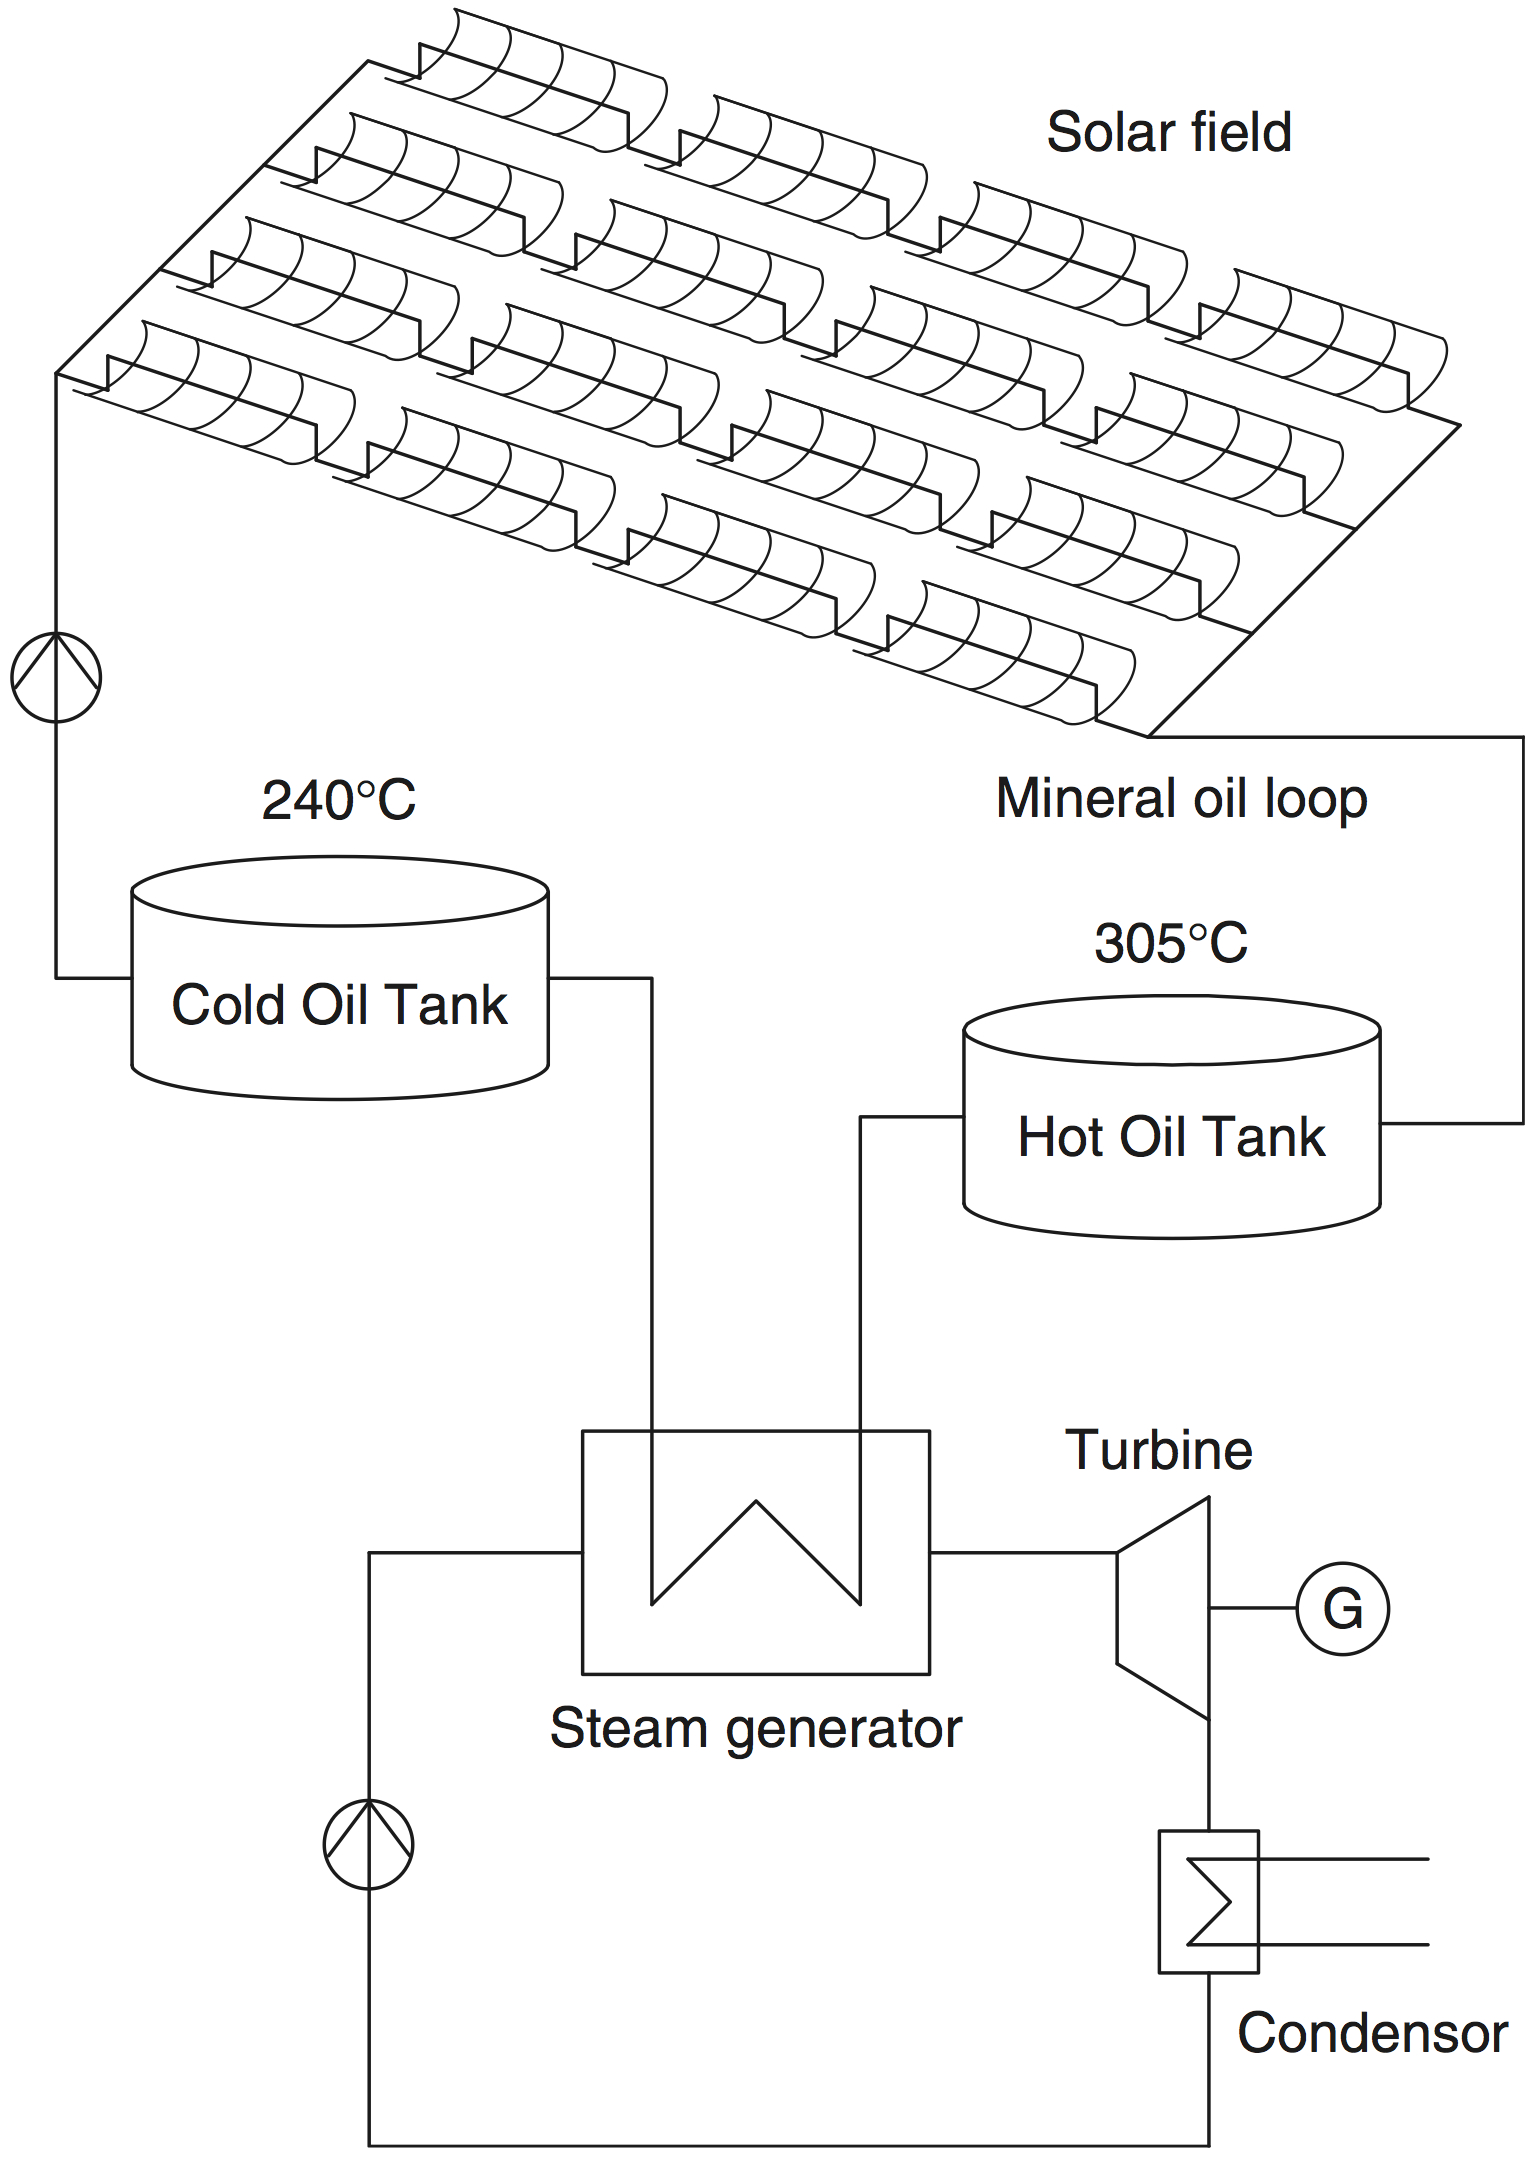
\includegraphics[width=0.6\textwidth]{FIG/troughdirecttwotank}
                \caption{SEGS-1 PTC plant with direct storage of heat transfer fluid.}\label{troughdirecttwotank}
        \end{subfigure}%
        ~
        \begin{subfigure}[b]{0.5\textwidth}
                \centering
                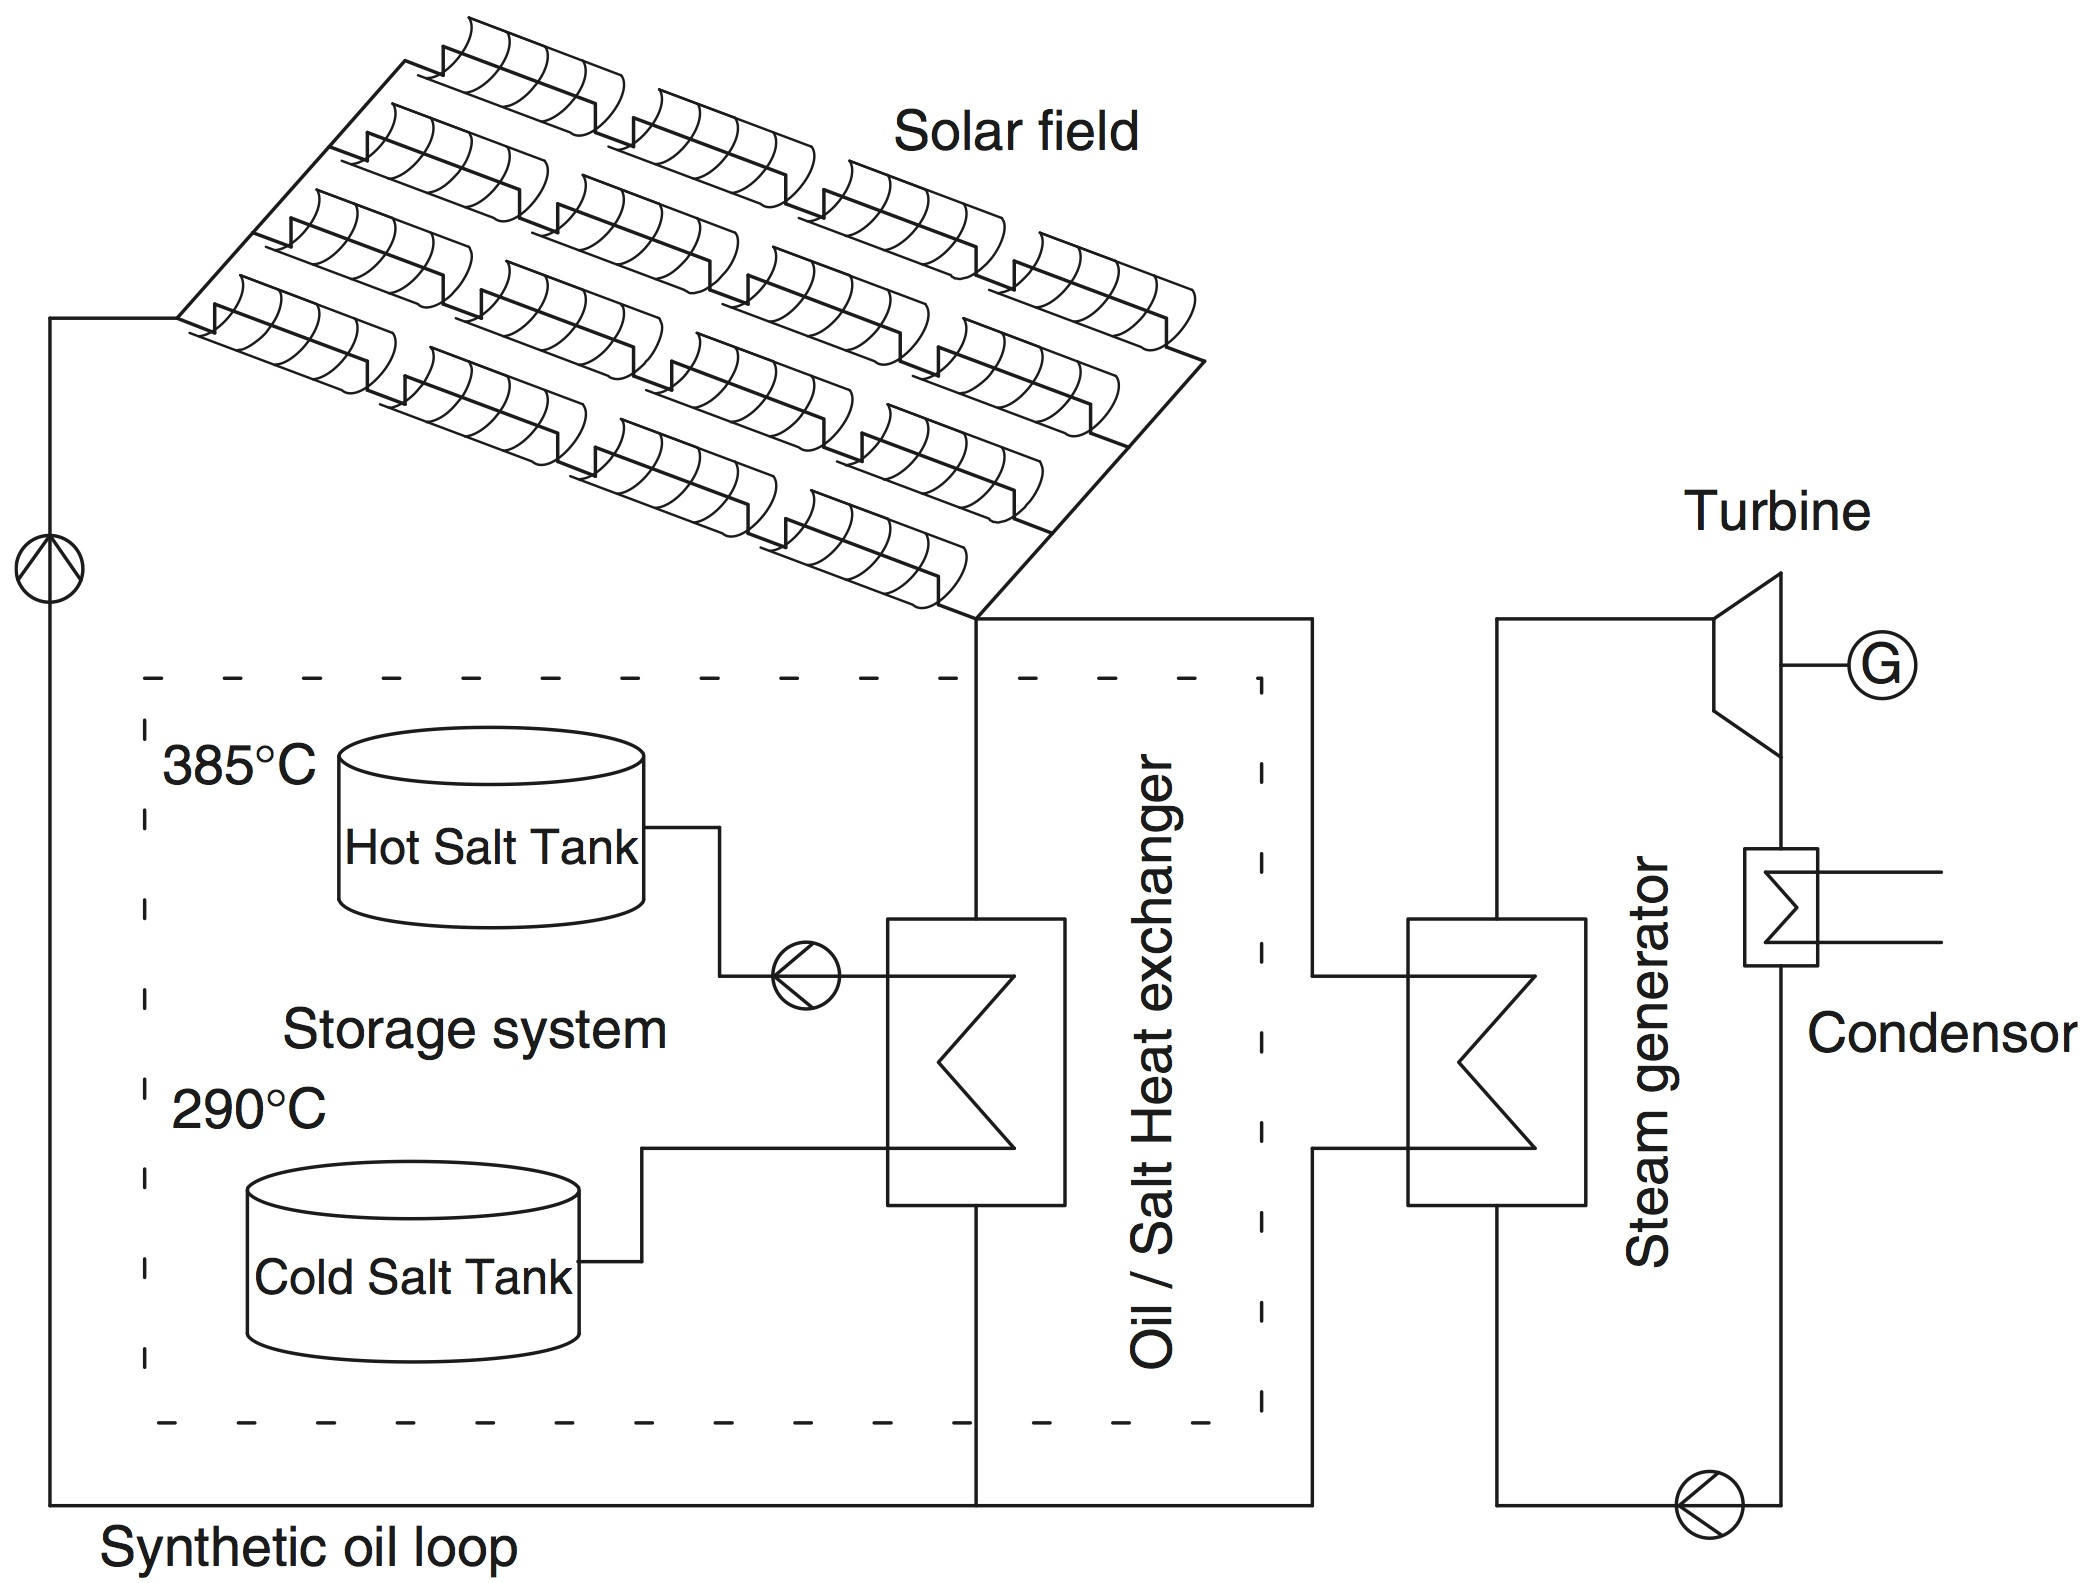
\includegraphics[width=1\textwidth]{FIG/troughtindirecttwotank}
                \caption{PTC power plant with indirect storage system using molten salt.}\label{troughtindirecttwotank}
        \end{subfigure}
        \caption[Simplified scheme of PTC power plants and storage concepts.]{Simplified scheme of PTC power plants and storage concepts \cite{Steinmann2012}.}\label{storageconceptstrough}
\end{figure}
\subsubsection{Indirect molten salt storage units}
Since the direct storage of the synthetic HTF is not attractive, an indirect storage concept was proposed. This should use a low cost storage medium, which can be stored at ambient pressure between 290$\,^{\circ}\mathrm{C}$ and 390$\,^{\circ}\mathrm{C}$. The use of molten nitrate salts was a nearby solution whose elements is considered and development since the early stage of CSP technology in the 1980's. Depending on the importance of material costs and there thermal stability, an sodium-nitrate-rich (NaNO$_3$) mixture containing 60\% NaNO$_3$ and 40\% KNO$_3$ (potassium nitrate) is preferred if an large quantities is required. The maximum temperature is in range of 550-580$\,^{\circ}\mathrm{C}$ and the melting temperature is in the range of 230$\,^{\circ}\mathrm{C}$. \cite{Richter2013}

Figure \ref{troughtindirecttwotank} shows a simplified scheme to implement a indirect two tank molten salt storage concept into a parabolic trough plant. Two separate insulated cylindrical thanks made of steel and carbon are used. Each tank can contain the total molten salt volume. Due to the temperature-dependent density of molten salt, the volume of the hot fluid tank has to be 4\% lager. To prevent freezing of molten salt an electrical immersion heaters are located at the bottom of the tanks.\cite{Kelly2006}.

The Andasol-1 facility, completed 2008 in Andalusia, Spain was the first commercial CSP plant using indirect molten salt storage. This plant can be operated for 7.5~h at 50~MW$_{el}$ by thermal energy provided by an indirect two-tank molten salt storage system. The molten salt storage fluid of 28~500~tons is cycled between 385$\,^{\circ}\mathrm{C}$ and 295$\,^{\circ}\mathrm{C}$, resulting a storage capacity of 1~050~MWh$_{th}$ \cite{Relloso2009}. The storage tanks have a height of 14~m and a diameter of 36~m. The similar CSP plants Andasol-2 and Andasol-3 started operation in 2009 and 2011. \cite{SolarMillenniumAG2008,NREL2008,NREL2013a,NREL2013}

Figure \ref{SolanaStorage} shows the Solana facility located in Arizona, USA. This plant was completed in 2013 and is the the largest parabolic trough plant so far. The indirect molten salt storage system uses 12 tanks to provide 280~MW$_{el}$ for a duration of six hours. \cite{AbengoaSolar2013a}

Since 2015 SA has also their first commercial CSP plant using indirect molten salt storage technology (Figure \ref{KaXu-solar-field}). KaXu Solar One is located next to Poffader in the Northern Cape and is a parabolic trough plant with 100~MW$_{el}$ capacity and 2.5~h of thermal storage in molten salts. \cite{NREL2015c}
\begin{figure}[!bhtp]  
\centering
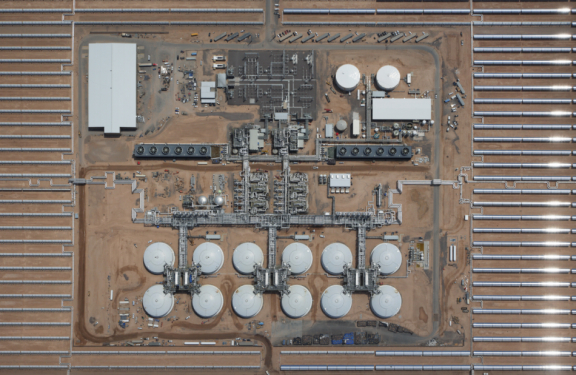
\includegraphics[width=0.9\linewidth]{FIG/SolanaStorage}
\caption[Overall view of Solana PTC facility with 12 storage tanks for molten salt.]{Overall view of Solana PTC facility with 12 storage tanks for molten salt \cite{AbengoaSolar2013}.}\label{SolanaStorage}
\end{figure}
\subsubsection{Steam accumulators}
In 2007 the first commercial CSP plant in Europe, the Planta Solar 10 (PS10) started near to Seville in Spain. The power tower uses saturated steam at 250$\,^{\circ}\mathrm{C}$ and 40~bar to drive a 11~MW$_{el}$ power circle. A schematic diagram of the PS10 is shown in Figure \ref{directsteamgeneration} on Page \pageref{directsteamgeneration}. The energy availability for storage is limited because the  plant is designed for a small solar multiple value of 1.3. Therefore a stream accumulator was selected as storage concept. The cross-sectional view of an steam accumulator is shown in Figure \ref{SteamAccumulatot}, which is also denoted as Ruths' storage or saturated steam storage. During charging the surplus stream is fed into a pressurized liquid water volume. The liquid water acts as storage medium. So the condensing steam increases the pressure and temperature of the liquid water in the volume. The storage is designed in horizontal cylindrical pressure vessel, whose volume is filled with 90\% saturated liquid and the remaining volume is filled by saturated stream. Saturated stream will provided during discharge by the steam accumulator. While the saturated steam is taken out of the steam accumulator is the pressure in the liquid volume declining. The saturated liquid volume generates thereby additional saturated steam by a reaction of the pressure reduction. Meanwhile the mass reduction of the liquid volume is usually in the range of 10-20\%. Pressure and temperature of the steam from the steam accumulator decline continuously during the discharge process. The PS-10 plant uses four separate tanks to store about 20~MWh$_{th}$ which is sufficient to produce 50\% load for 50 minutes. Attractive features of steam accumulators are their robustness and the simplicity of the concept. The fast reaction time makes the steam accumulator to an prefer storage concept of buffer storage solution intended for short fluctuation of solar radiation. But significant exergy losses occur due to the temperature difference between the steam and liquid volume during the charging. While steam accumulators are an attractive solution for small and medium sized solar process heat application, W.-D. Steinmann from the German Aerospace Center (DLR) \cite{Steinmann2015} has the opinion they are not expected to play a major role in the future of CSP applications. \cite{Richter2013}

Nonetheless the first power tower in SA, Khi Solar One will use super-heated steam, dry cooling technology, and a 2~h steam storage system. Khi Solar One is a 50 MW solar power tower plant being built by Abengoa near the town of Upington in the Northern Cape Province. Operation was scheduled to begin in 2014 but is still under construction (Status Oct. 2015). \cite{Abengoa2014,NREL2014}

\begin{figure}[!htbp]  
\centering
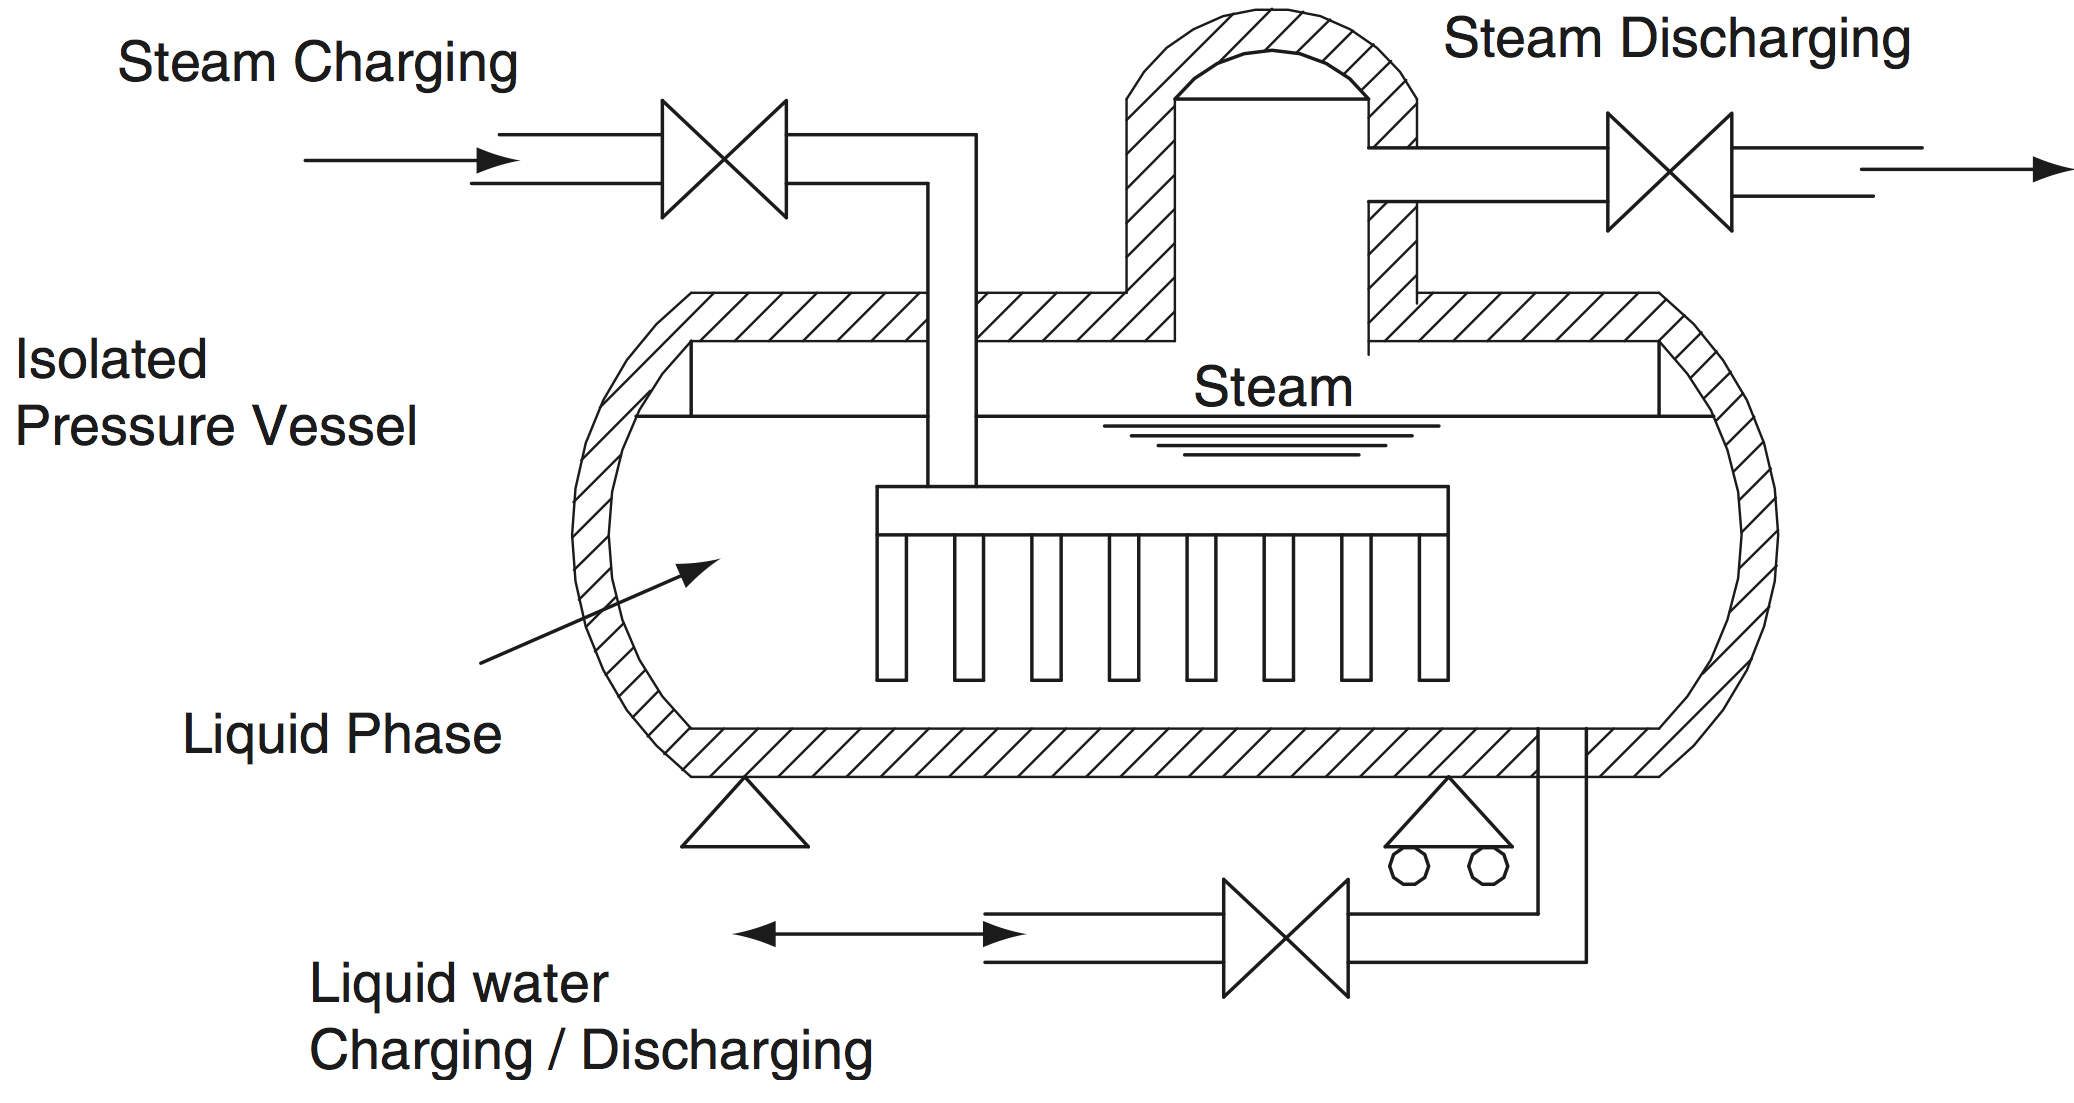
\includegraphics[width=0.7\linewidth]{FIG/SteamAccumulatot}
\caption[Scheme of a steam accumulator.]{Scheme of a steam accumulator \cite{Steinmann2006}.}\label{SteamAccumulatot}
\end{figure}
\subsubsection{Direct molten salt storage units}
Increasing the maximum process temperature of the thermal cycle of an CSP plant seams to be an efficient way to improve the economics of solar thermal electricity generation. A higher maximum process temperature allows also to increase the thermal storage cycle temperature, which has an significant impact on the specific storage capacity for sensible heat. Thereby the required storage inventory and the volume of the storage tanks can be reduced. Also less electric power for pumping the storage medium is required. But on the other hand, increasing with the higher temperature as well corrosion problems and thermomechanical stress.
\begin{figure}[t!]  
\centering
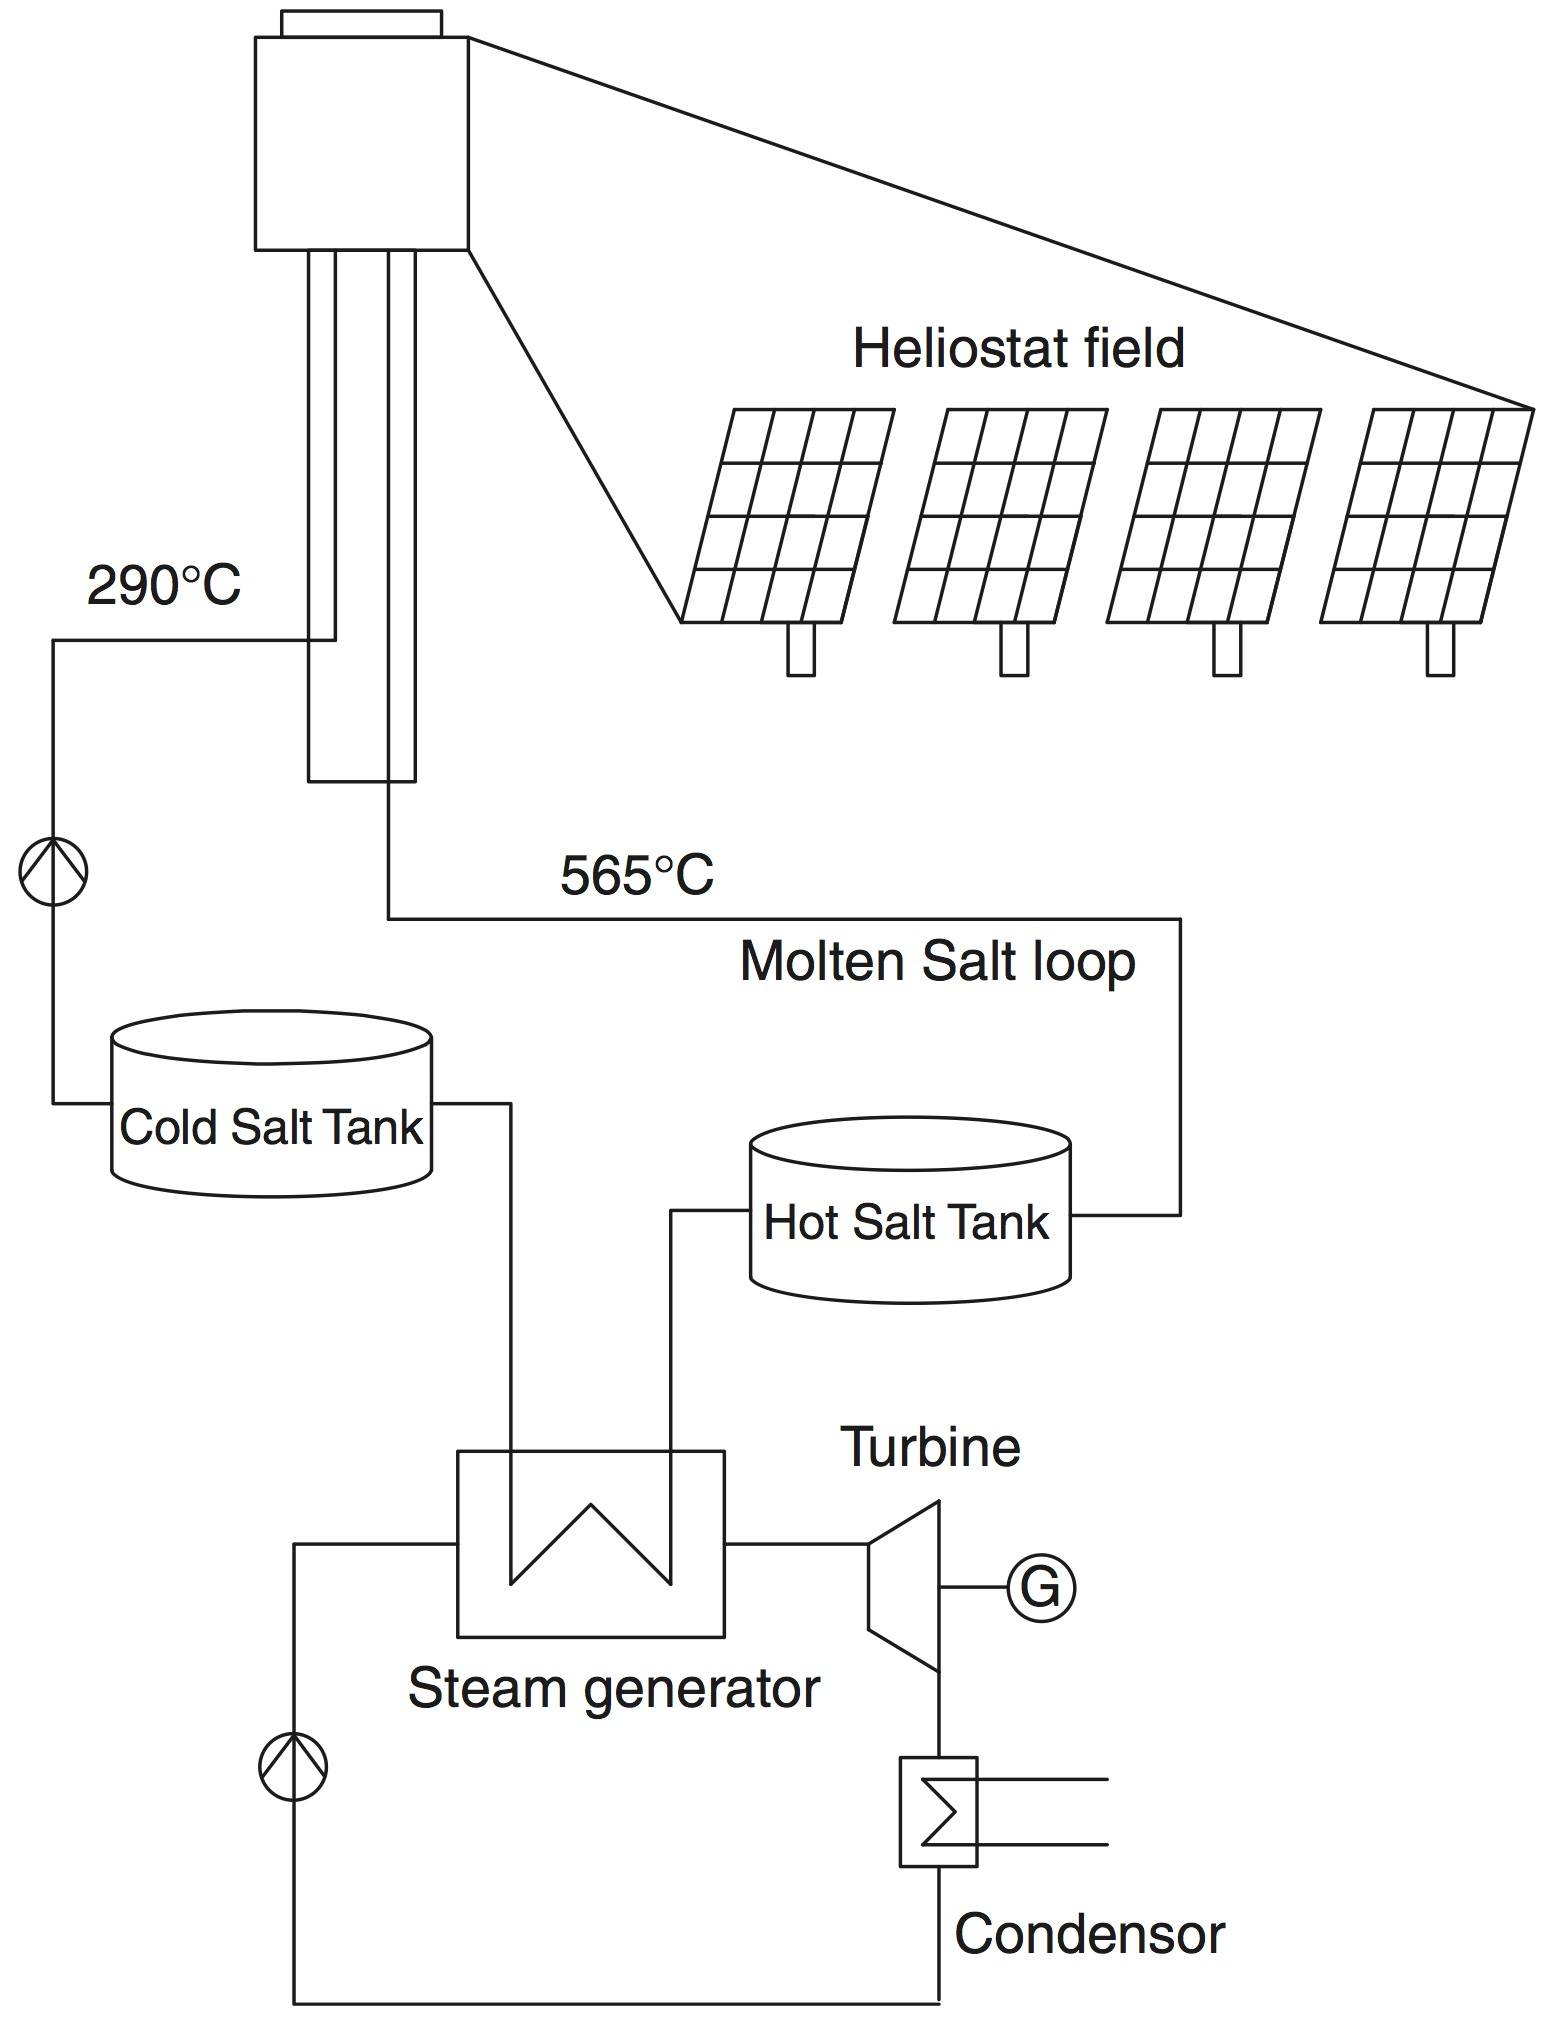
\includegraphics[width=0.45\linewidth]{FIG/towerdirecttwotank}
\caption[Simplified scheme of Solar Two CRS power plant with direct storage of molten salt used as heat transfer fluid.]{Simplified scheme of Solar Two CRS power plant with direct storage of molten salt used as heat transfer fluid \cite{Richter2013}.}\label{towerdirecttwotank}
\end{figure}


Using the solar central receiver concept is an opportunity to raise the temperature of the process up to more than 565$\,^{\circ}\mathrm{C}$. Figure \ref{towerdirecttwotank}  shows a simplified scheme of direct two-tank molten salt storage concept integrated into CRS. This concept was first tested in the Solar Two power plant. This pilot solar-thermal project was built in the Mojave Desert just east of Barstow, CA, USA in 1994 on basis of the Solar One facility and was operating until 1999. A 10~MW$_{el}$ Rankine cycle was connected to the central receiver providing 35~MW$_{th}$. The two-tank storage system had an inventory of 1~400~t of a mixture of molten sodium nitrate (60\% by weight) and potassium nitrate (40\% by weight), with a total volume of about 1~700~m$^3$. The capacity of the storage system was 107~MWh$_{th}$ and operated between 565$\,^{\circ}\mathrm{C}$ and 290$\,^{\circ}\mathrm{C}$, which allowed the operation of the turbine for 3~h. The external isolated tanks had both a diameter of 11.6~m, the hot tank was mad of stainless steel had a height of 8.4~m with thermal loss in the range of 100~kW, the cold tank made of carbon steel was 7.8~m tall and transferred about 50~kW to the environment. The Solar Two project also gained the operational experience for handling larger quantities of nitrate salt for storage applications. Although, their was some changes observed in the physical properties of molten salt during the duration of the project, their was no problems resulted. After the 30~000~h project test and the analyses of the construction material, it was concluded that salt-induced no practical limitation on the useful life of tanks. Also the nitrate salt was recycled for use as fertilizer at the end of the project. \cite{Steinmann2015} 

The first commercial solar tower plant using molten salt with a direct storage system is Gemasolar, which was commissioned in 2011. It uses the first high-temperature solar receiver with molten salt, which provides 15 hours of thermal storage and an annual capacity factor of about 75\%. The size of the storage allows the plant to operate 24~h per day. The facility generates 19.9~MW$_{el}$ from 2~650~heliostats each 120~m$^2$ aperture area. The technology is based on the Solar Two and has the same temperature difference in the receiver from 275~K. \cite{NREL2011}

The Atacama-1, which is currently under construction in the Atacama desert in Chile, will also use a direct storage in molten salt for 17.5~h of storage. \cite{NREL2015b,AbengoaSolar2015a,AbengoaSolar2015}

Also parabolic trough power plants using direct molten salt storage units. The commercial used Archimede solar power plant in Italy is the first parabolic trough plant using molten salt as HTF. It started 2010 the production with 5~MW turbine capacity. The storage capacity reaches for 8 hours and has a total mass of 1~580~t of molten salt. With a tank size of 6.5~m in height and 13.5 m in diameter, the capacity is 100~MWh$_{th}$. \cite{NREL2012}



In a nutshell, the direct or indirect two-tank molten salt storage technologies are represent current state of art for commercial large-scale CSP applications. While this concepts shows a low technical and environmental risk, the potential for cost reduction is limited here. 
\subsection{Power cycles for CSP systems} \label{subsection_powerblock}
As mentioned in the overview of solar power technologies in Figure \ref{OverviewSTP} on Page \pageref{OverviewSTP}, a range of different solar to electric energy conversion systems can be applied. Commonly used as conversion systems in current large-scale CR and PTC applications are steam turbines which are based on the Rankine cycle. Nearly all convectional fired power plants using the Rankine cycle to convert heat in electricity. If an conventional fired combined cycle power plant is supplemented with a CSP system it uses an integrated solar combined cycle (ISCC), which is also based on the Rankine cycle. An additional conversion systems for CRS and parabolic dishes is the Brayton cycle (also known as Joule cycle). However, for efficient cycle operation temperatures of 1~000$\,^{\circ}\mathrm{C}$ are needed. Therefore the Brayton cycle has just been operated in demonstration CSP systems. CSP systems also uses Organic Rankine cycles, Stirling engines and other opportunities to generate electricity. \cite{Lovegrove2012}



A CSP plant with Rankine cycle is basically working in four steps using a steam turbine:
\begin{itemize}
\item Compressing pure feed water to high pressure. 
\item Pre-heating, boiling and superheating steam in a boiler which may be in the focal point, or may be heated using a heat exchanger with another HTF. 
\item Expanding the steam to low pressure via a series of turbines that drive a generator.
\item At the end of the expansion process, condensing the low pressure steam, with the aid of a cooling tower and then re-using it in the cycle.
\end{itemize}
\newpage
\section{Large scale PV power plants}\label{Large scale photo voltaic (PV) power plants}
two axis tracking PV
\subsection{Large-scale PV power plants}

\subsection{Large-scale electrical energy storage systems}
electrical energy storage (EES)
EESSchema
\begin{figure}[htbp]  
\centering
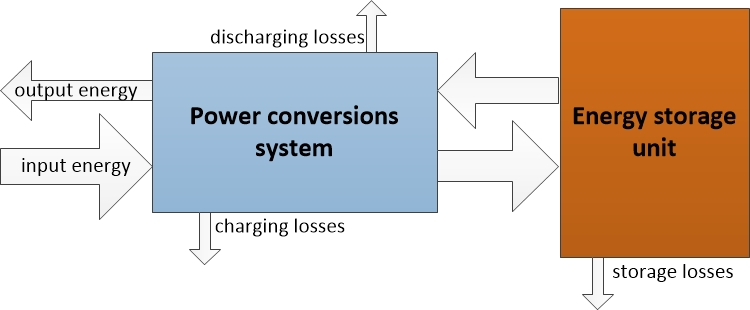
\includegraphics[width=0.65\linewidth]{FIG/EESSchema}
\caption[Schema of an electrical energy storage (EES) system and there energy losses.]{Schema of an electrical energy storage (EES) system and there energy losses.}\label{TCC_EES}
\end{figure}

\begin{equation}
\textrm{Overall storage efficiency (AC-to-AC)} =\frac{E_{out} \textrm{ (kWh)} }{E_{in} \textrm{ (kWh)}}
\end{equation}

\begin{figure}[htbp]  
\centering
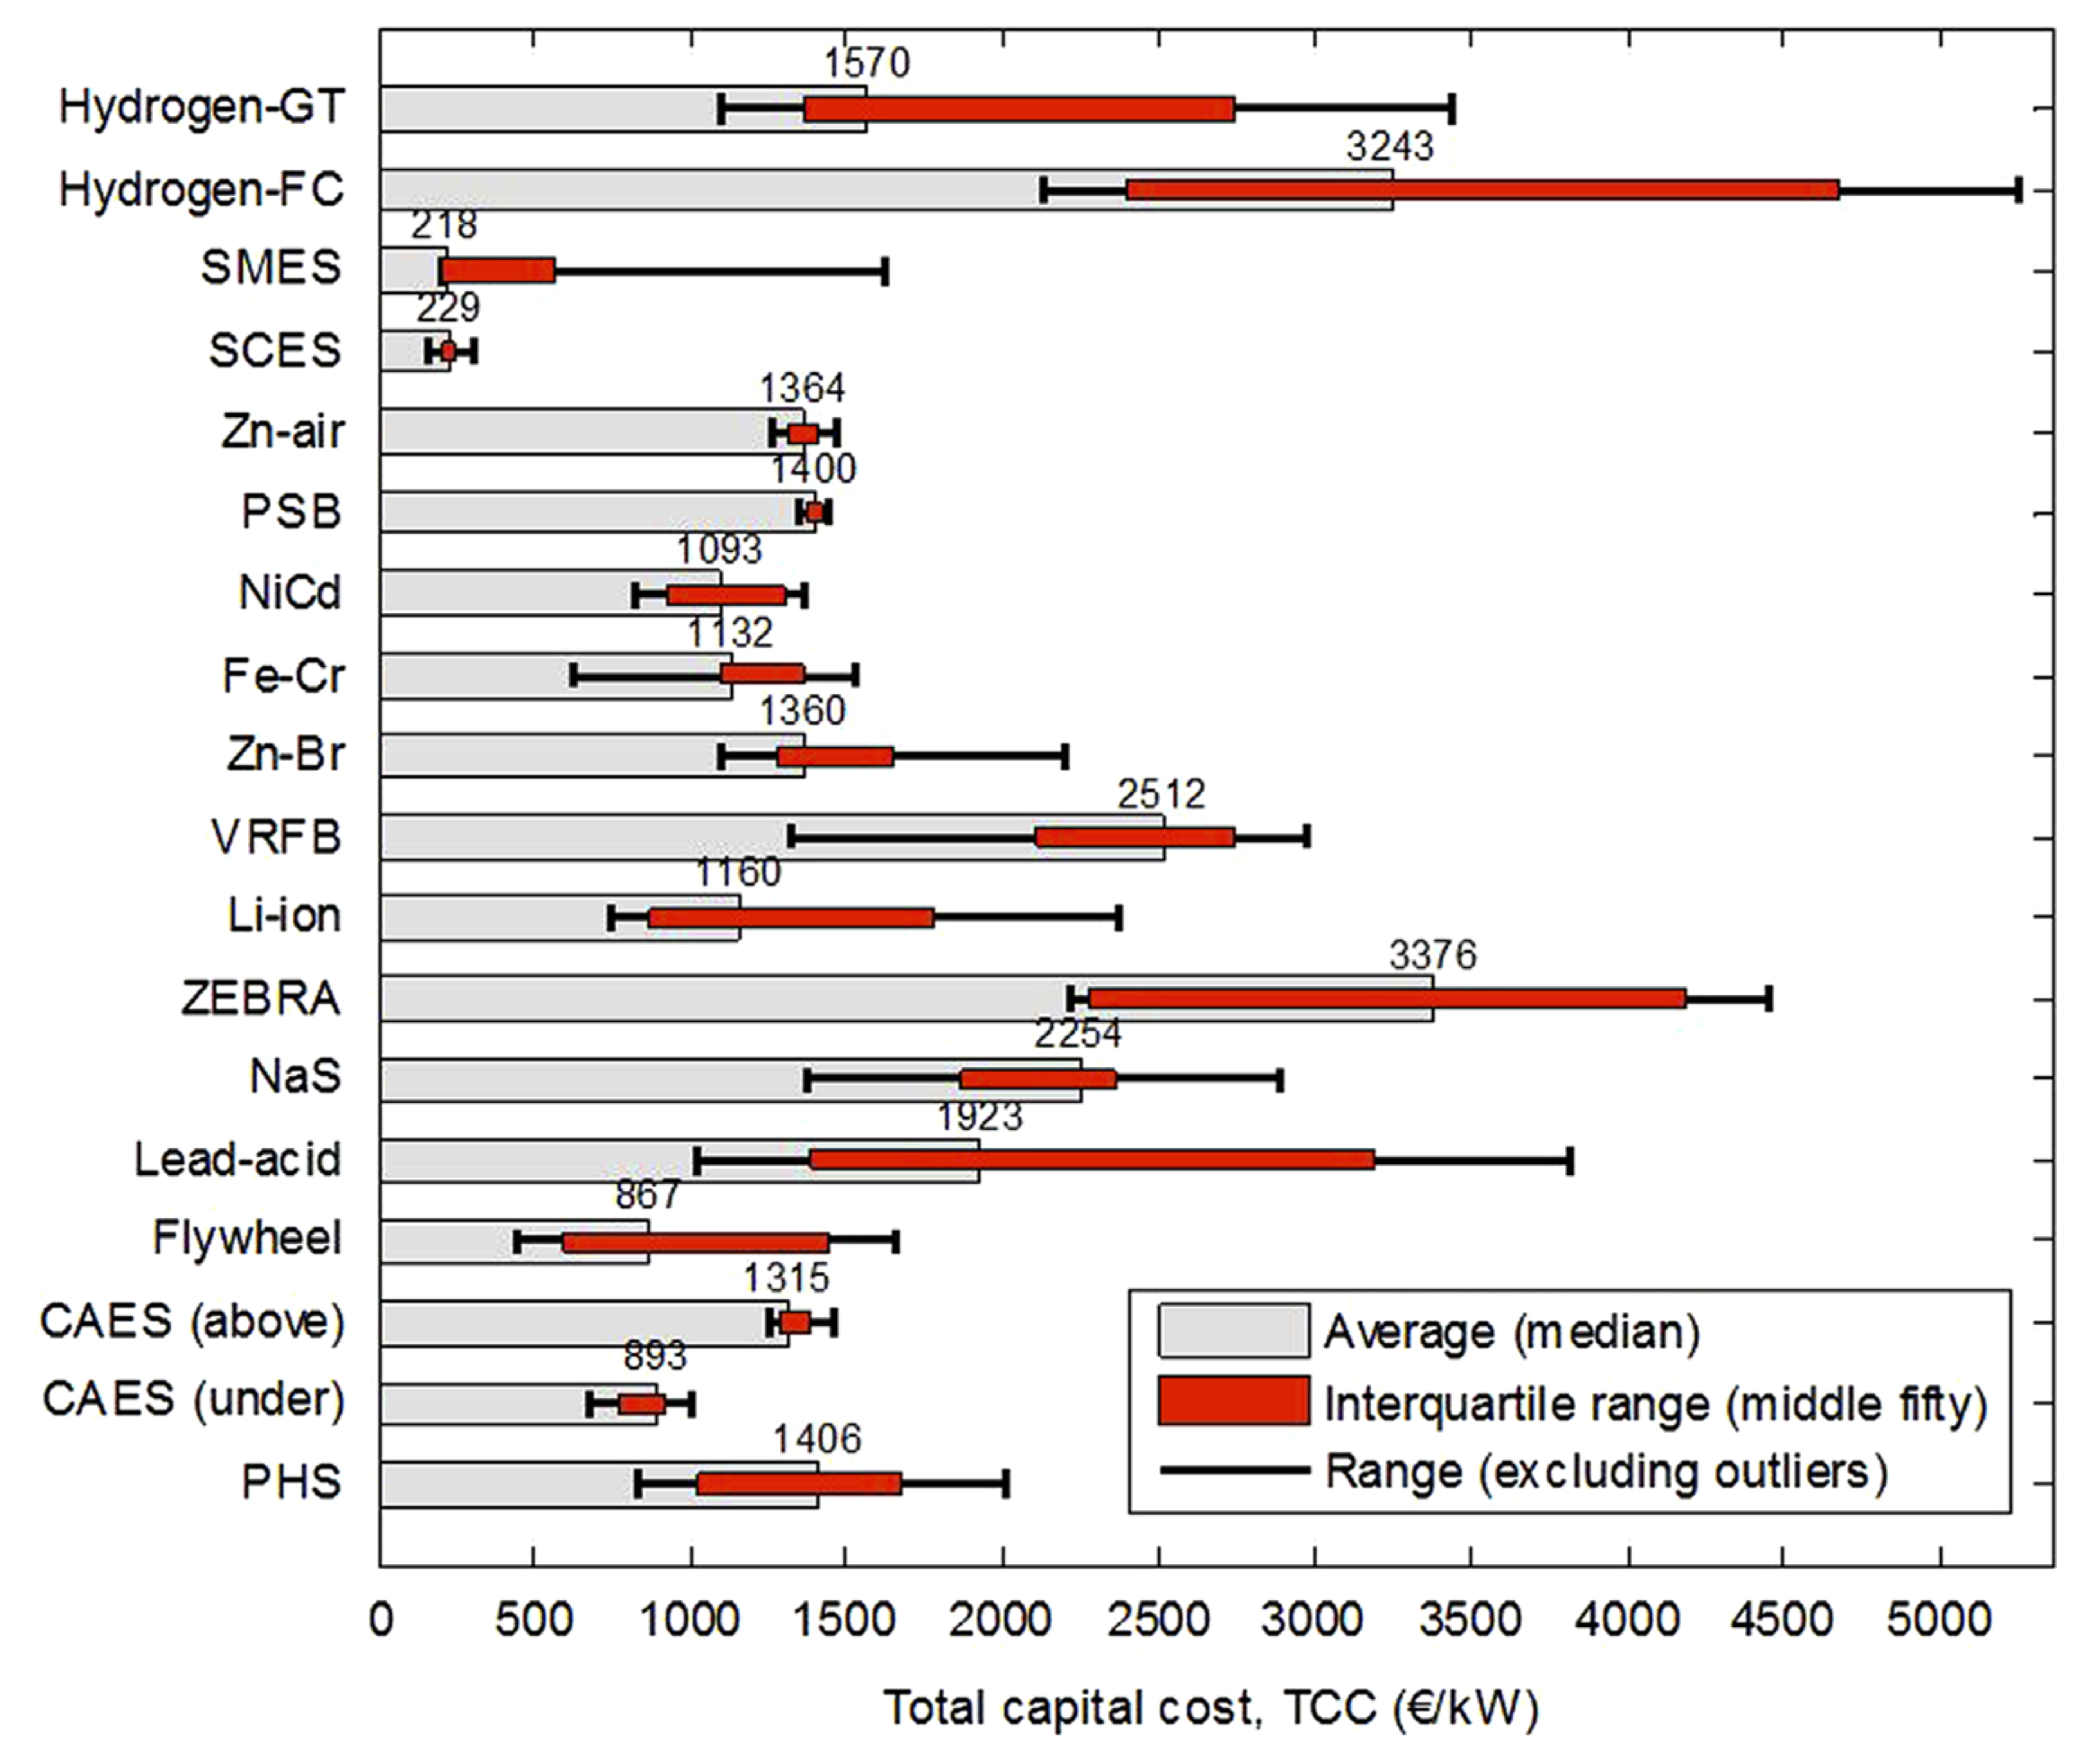
\includegraphics[width=0.75\linewidth]{FIG/TCC_EES}
\caption[Total capital cost in Euro (€) of large-scale EES systems per unit of nominal power rating including costs of power electronics, storage part, fixed obtain and maintainence and maybe incidental replacement costs.]{Total capital cost in Euro (€) of large-scale EES systems per unit of nominal power rating including costs of power electronics, storage part, fixed obtain and maintainence and maybe incidental replacement costs \cite{Zakeri2015}.}\label{TCC_EES}
\end{figure}

\section{Environmental impacts of CSP and PV}
Co2

Water use in O \& M

land use

energy use in operation and building
\cite{EASAC2011}

\cite{Caldes2012} 

\section{Chapter summary}

\pagebreak
